%!TEX root = ./template-skripsi.tex
%-------------------------------------------------------------------------------
%                            	BAB IV
%               		HASIL DAN PEMBAHASAN
%-------------------------------------------------------------------------------

\chapter{HASIL DAN PEMBAHASAN}

\section{Pra-Processing Citra}
\subsection{Input Gambar dan Penghilangan Background}

\begin{figure}[H]
    \centering
    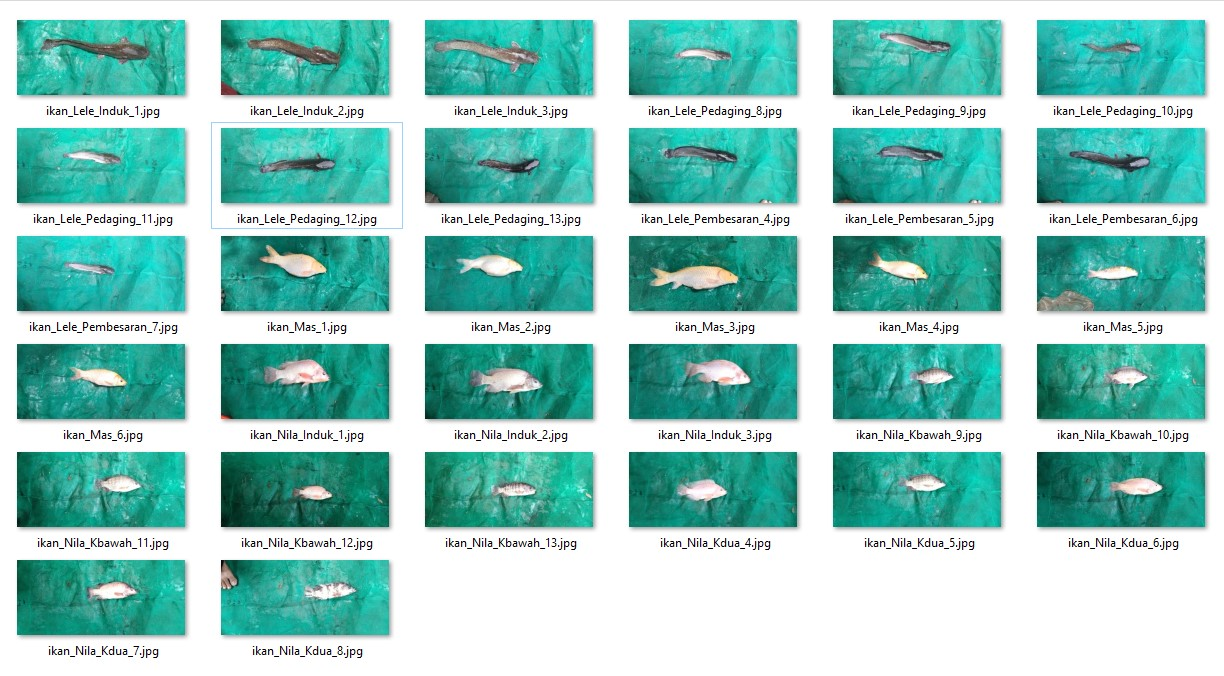
\includegraphics[width=0.8\textwidth]{gambar/Screenshot_3.jpg}
    \caption{Gambar yang akan digunakan dalam penelitian}\label{fig:folder-ikan}
\end{figure}

Langkah pertama yang dilakukan dalam penelitian adalah dengan memasukan \emph{dataset} untuk dilakukan \emph{pra-processing}. Dalam hal ini, gambar akan diberikan nama sesuai dengan jenis ikan, yaitu Ikan Mas, Ikan Lele, dan Ikan Nila.
\emph{pra-processing} dilakukan untuk memudahkan proses ektraksi sudut pada citra. \emph{pra-processing} terbagi menjadi beberapa tahapan, yaitu penghilangan background, rotasi citra berdasarkan sudut PCA, dan smoothing citra dengan Gaussian blur.
Berikut \emph{Source Code} yang digunakan dalam proses penghapusan background:

\begin{figure}[H]
    \begin{lstlisting}[language=Python, basicstyle=\tiny]
        remove(image, bgcolor=(255, 255, 255))    
    \end{lstlisting}
    \caption{\emph{source code}: Untuk menghapus background dari library rembg}
\end{figure}

Fungsi \emph{remove} digunakan untuk menghapus background dari gambar dengan menggunakan library \emph{rembg}. Parameter \emph{bgcolor} digunakan untuk menentukan warna background yang akan dihapus, dalam hal ini adalah warna putih dengan nilai RGB (255, 255, 255). Setelah fungsi ini dijalankan, gambar akan memiliki background transparan sehingga memudahkan proses ekstraksi sudut pada citra.

\begin{figure}[H]
	\centering
	\begin{subfigure}{.3\textwidth}
		\centering
        
\includegraphics[keepaspectratio, width=3cm]{gambar/IMG_20240121_131125.jpg}
		\caption{Ikan Mas}
	\end{subfigure}
	\begin{subfigure}{.3\textwidth}
		\centering
		
\includegraphics[keepaspectratio, width=3cm]{gambar/IMG_20240121_132544.jpg}
		\caption{Ikan lele}
	\end{subfigure} 
	\begin{subfigure}{.3\textwidth}
		\centering
		
\includegraphics[keepaspectratio, width=3cm]{gambar/IMG_20240121_140044.jpg}
		\caption{Ikan Nila Merah}
	\end{subfigure}
	\caption{Contoh Gambar dan Jenis Ikan yang Digunakan}\label{fig:dataset}
\end{figure}

\begin{figure}[H]
	\centering
	\begin{subfigure}{.3\textwidth}
		\centering
        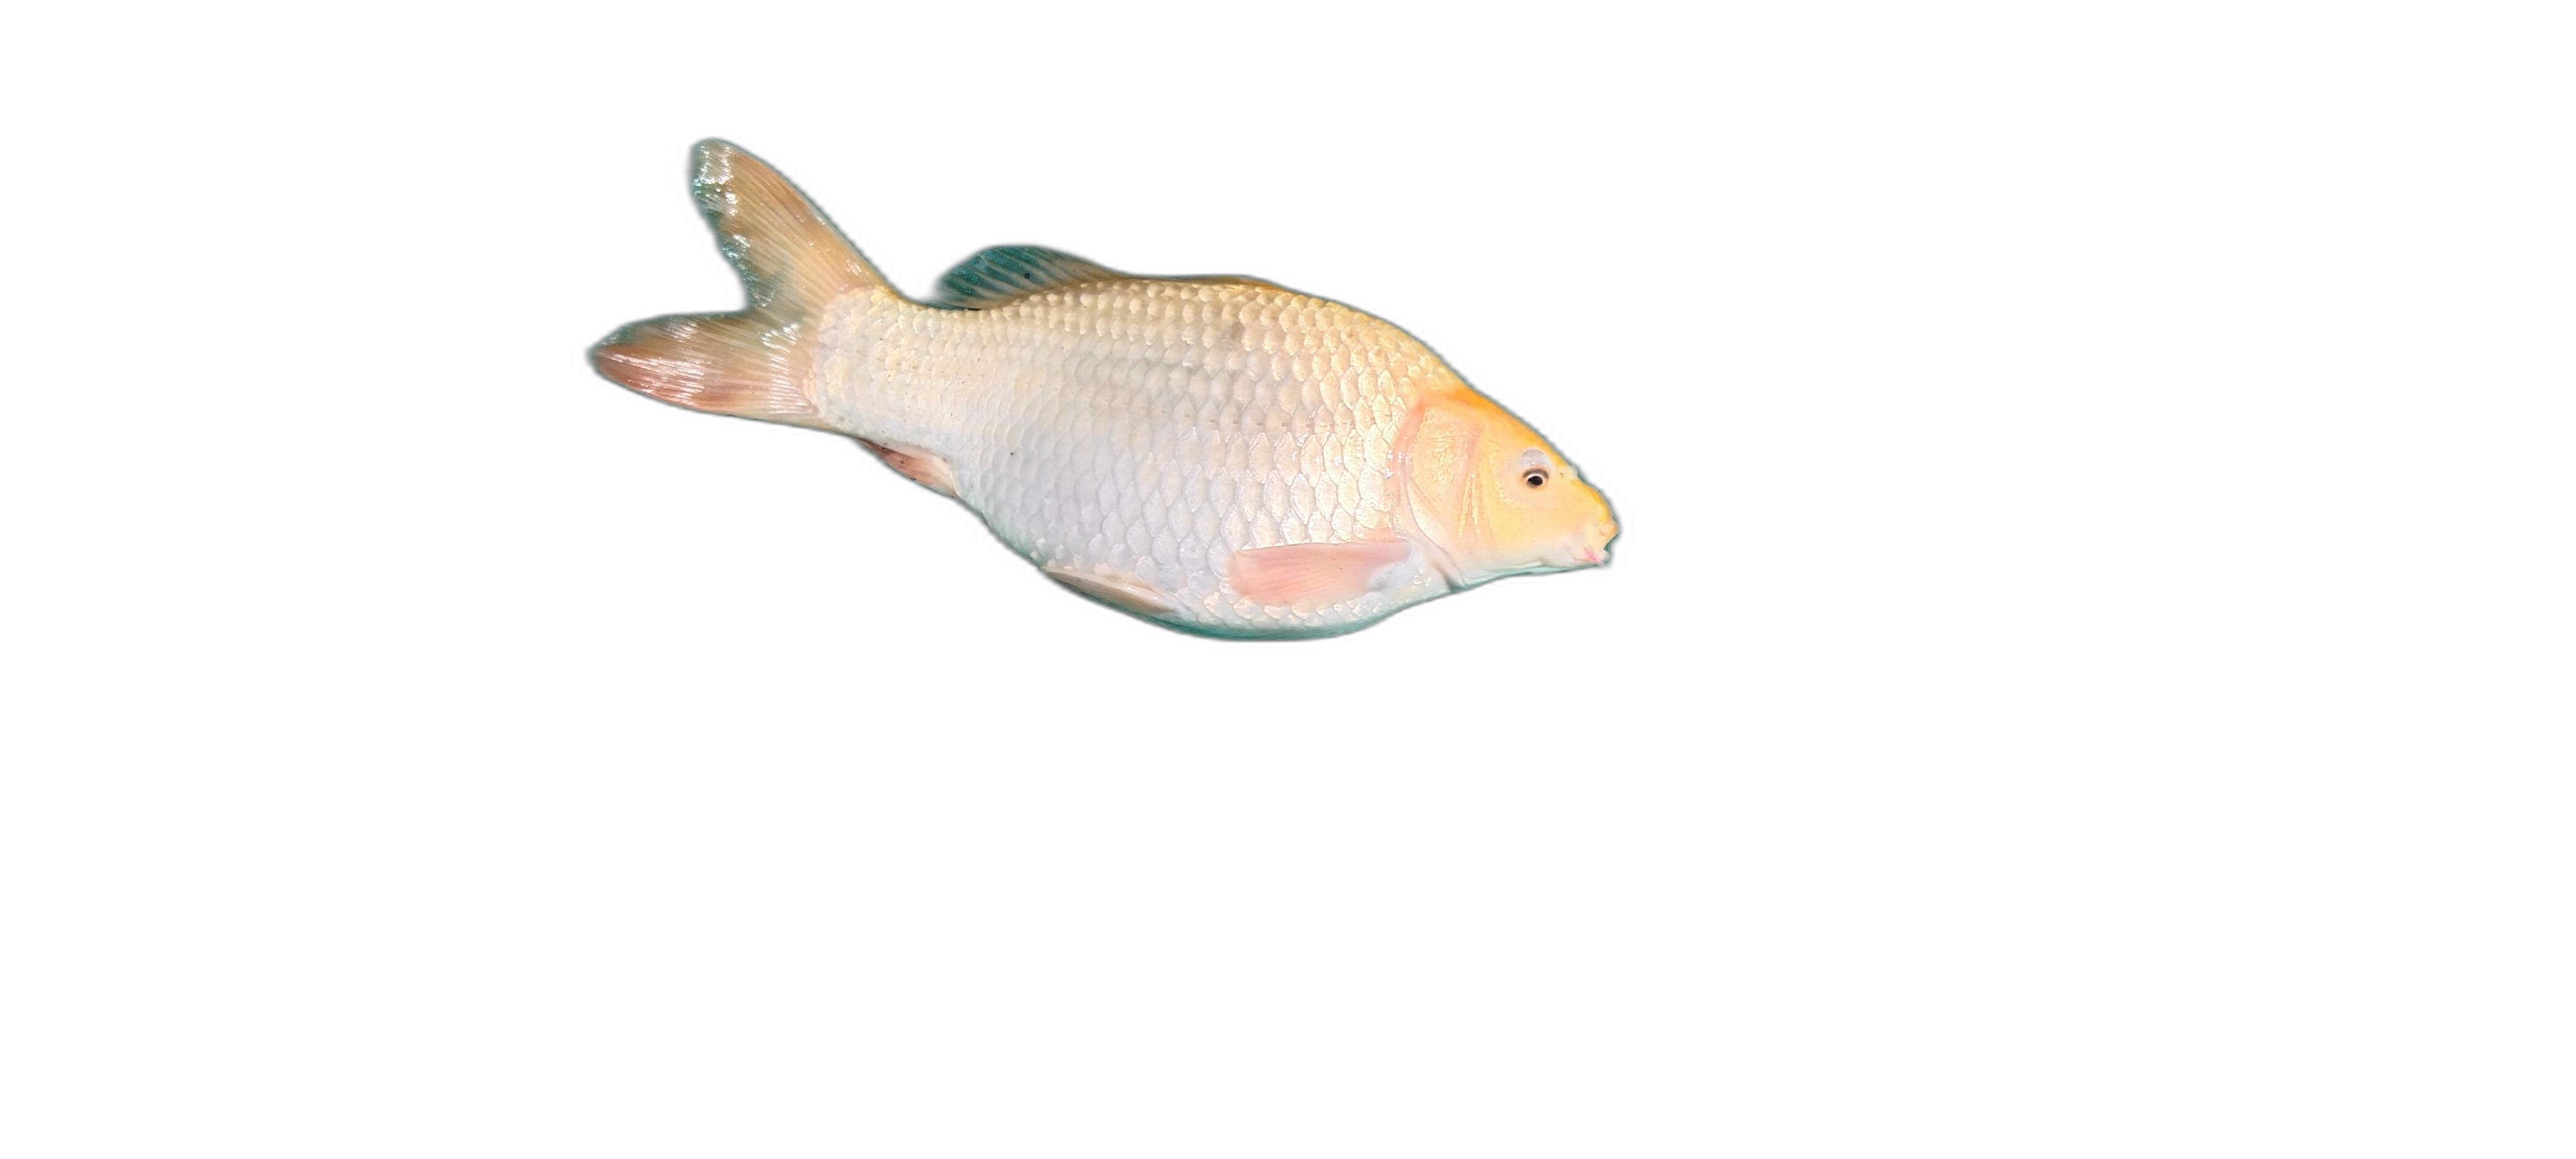
\includegraphics[keepaspectratio, width=3cm]{gambar/IMG_20240121_131125 - Copy.jpg}
		\caption{Ikan Mas}
	\end{subfigure}
	\begin{subfigure}{.3\textwidth}
		\centering
		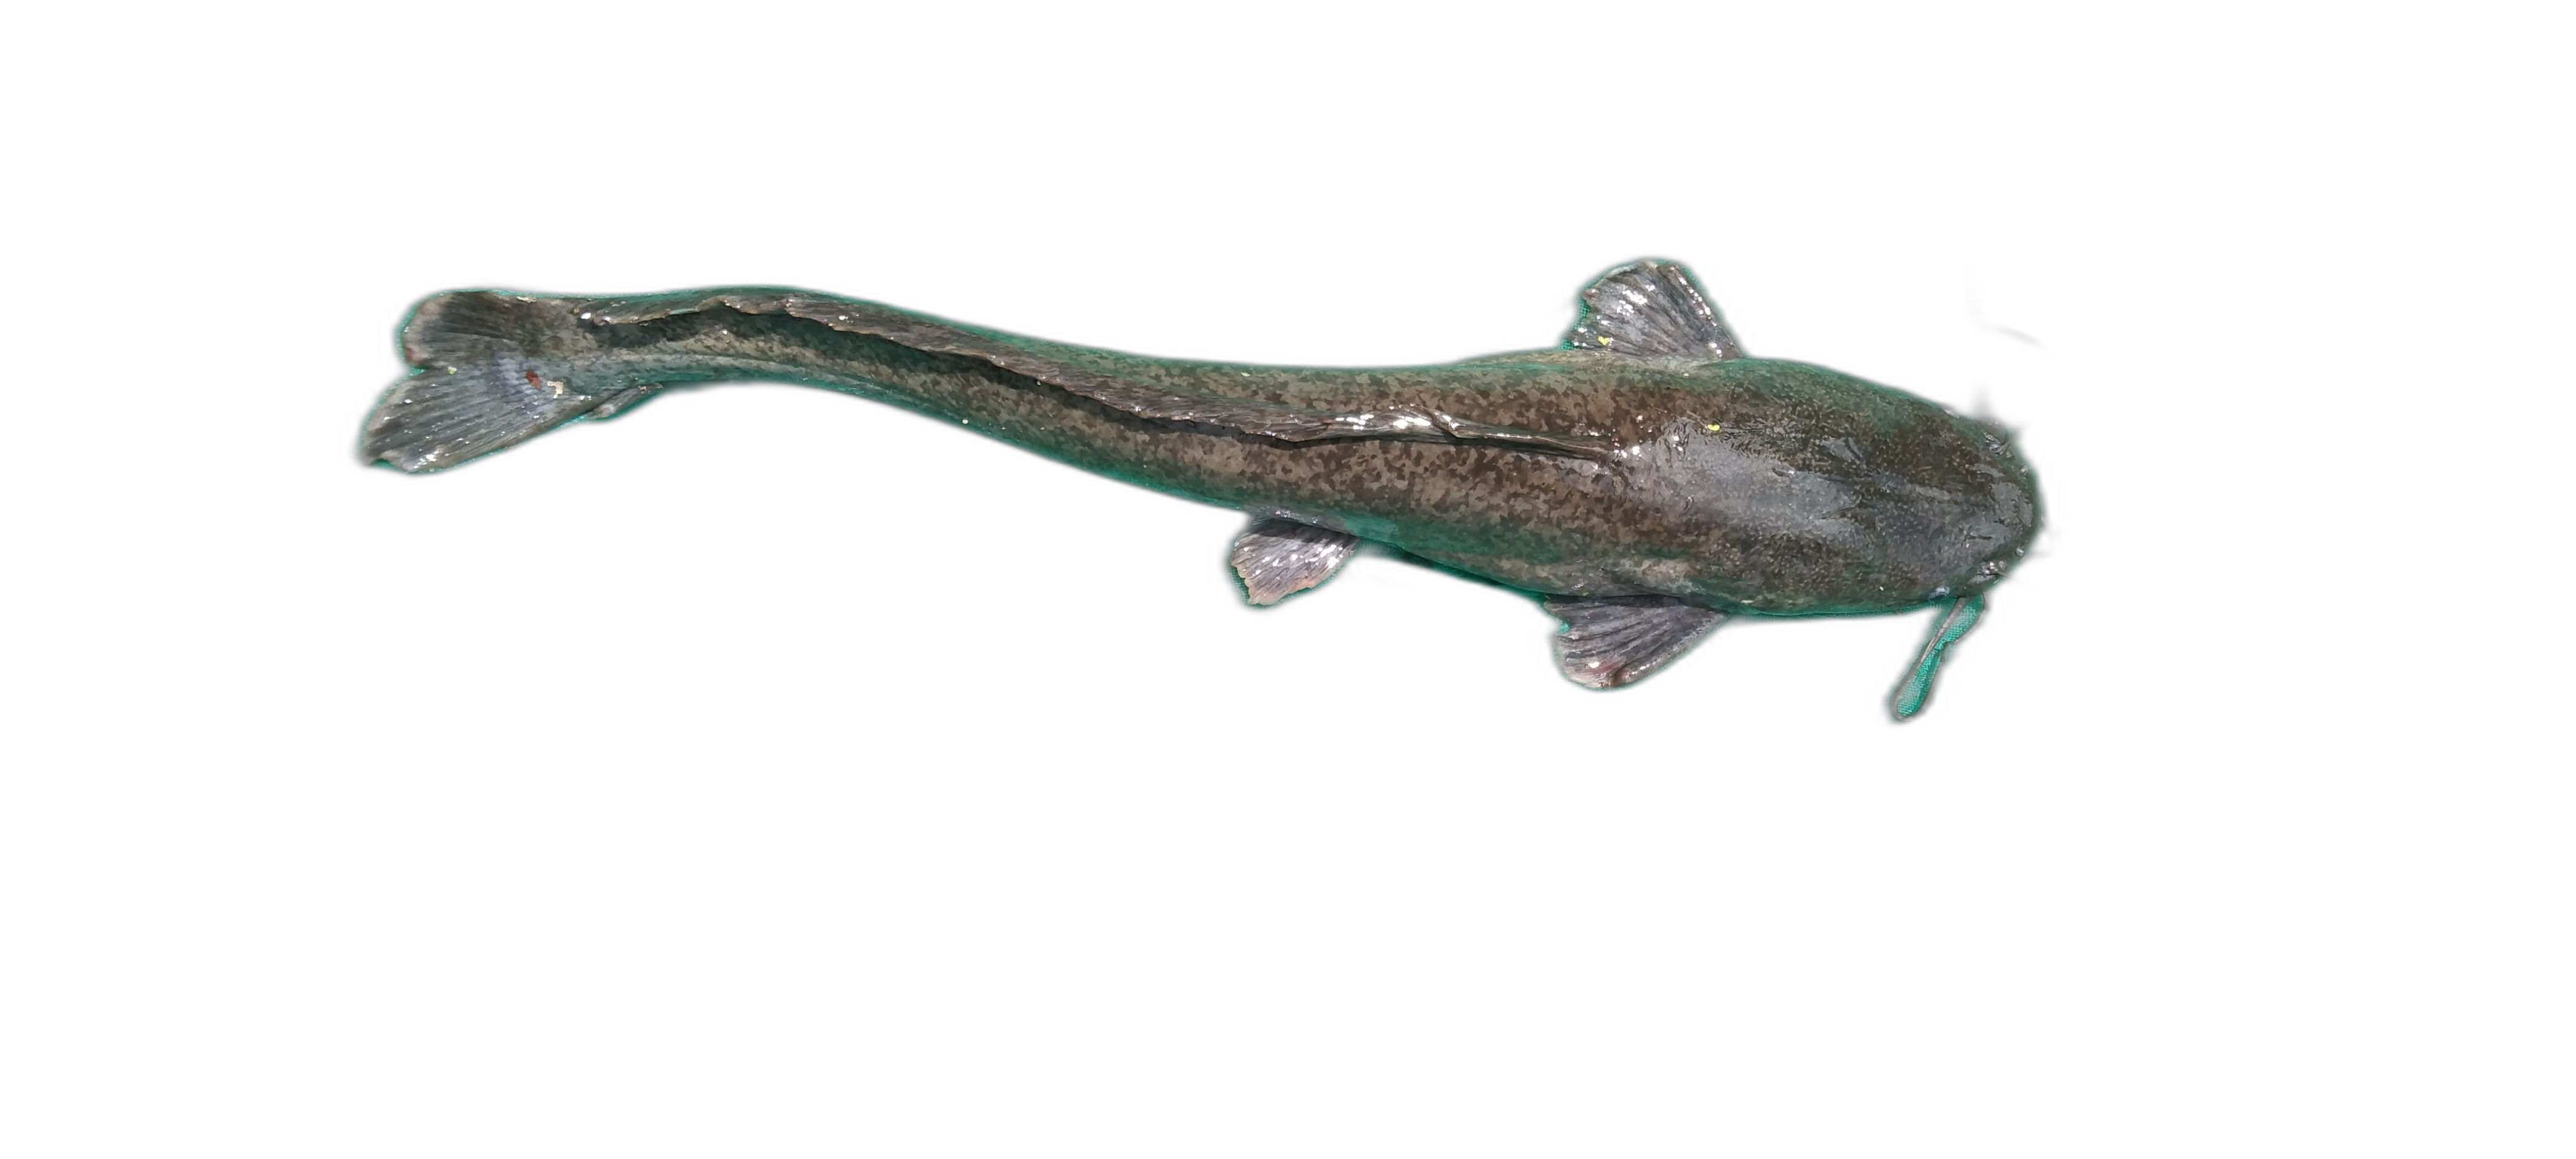
\includegraphics[keepaspectratio, width=3cm]{gambar/IMG_20240121_132544 - Copy.jpg}
		\caption{Ikan lele}
	\end{subfigure} 
	\begin{subfigure}{.3\textwidth}
		\centering
		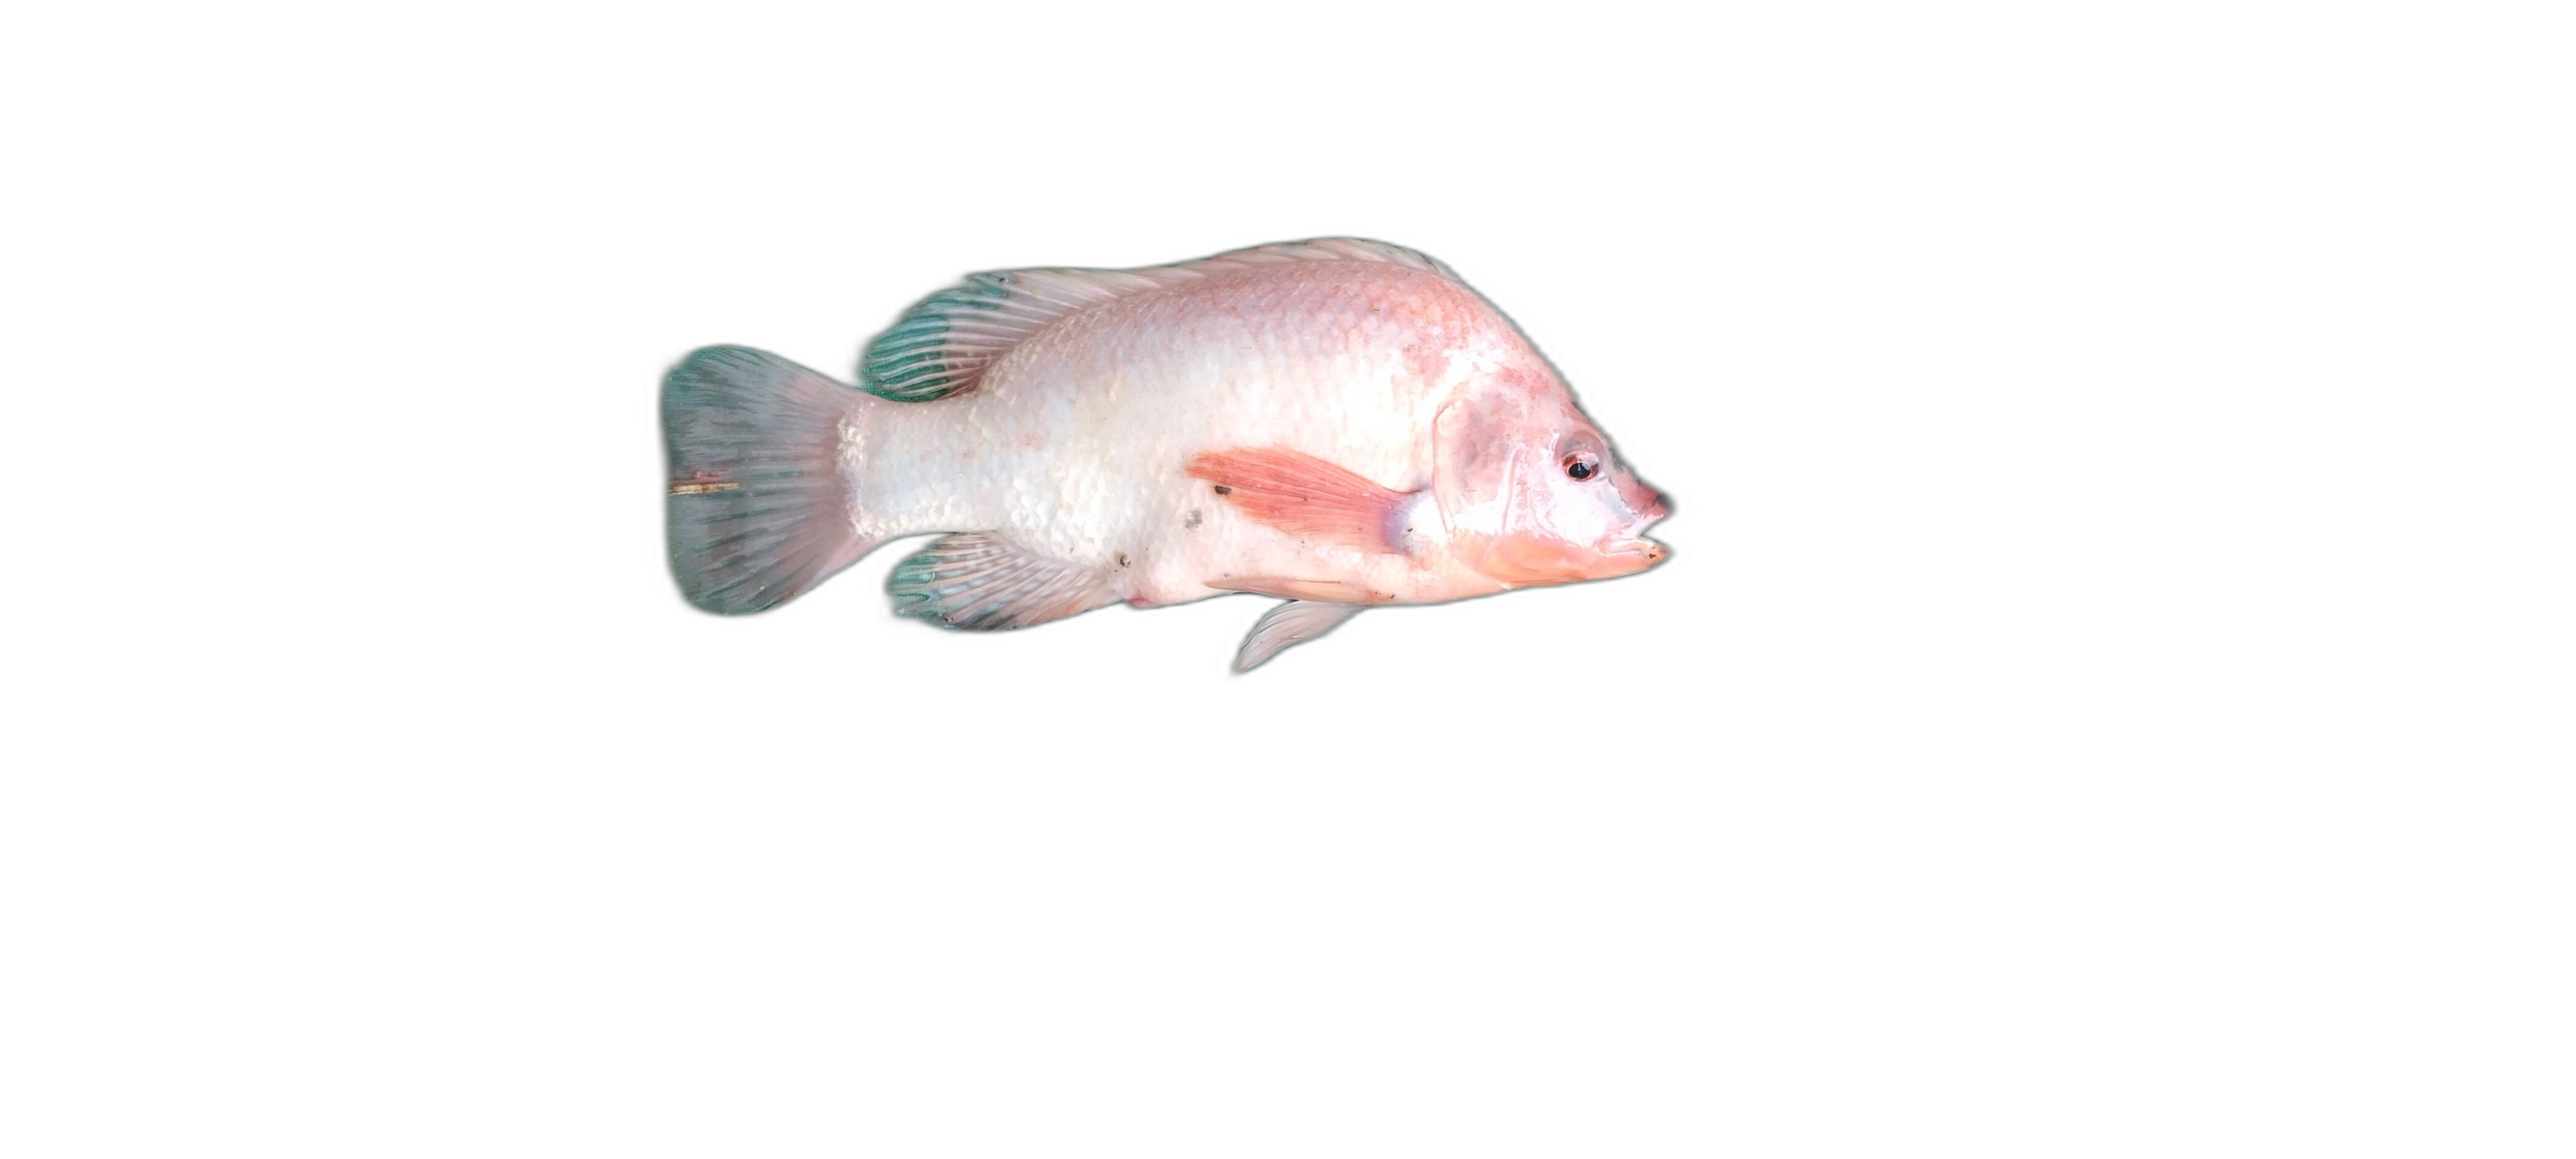
\includegraphics[keepaspectratio, width=3cm]{gambar/IMG_20240121_135842 - Copy.jpg}
		\caption{Ikan Nila Merah}
	\end{subfigure}
	\caption{Contoh hasil gambar yang telah dihilangkan backgroundnya}\label{fig:rembg}
\end{figure}
\subsection{Rotasi}

\begin{figure}[H]
    \begin{lstlisting}[language=Python, basicstyle=\tiny]
        def PCA_rotate(corners):
            if corners is not None and len(corners) > 0:
                
                pts = corners[:, [1, 0]].astype(np.float32)

                mean, eigenvectors, eigenvalues = cv2.PCACompute2(pts, mean=None)
                vx, vy = eigenvectors[0]

                pca_angle = np.degrees(np.arctan2(vy, vx))
                return pca_angle
        
        def PCa_rotate_image(image, corners):
                angle = PCA_rotate(corners)
                h, w = image.shape
                center_img = (w // 2, h // 2)

                rotation_matrix_pca = cv2.getRotationMatrix2D(center_img, angle, 1.0)
                rotated_img_pca = cv2.warpAffine(image, rotation_matrix_pca, (w, h), borderValue=(255, 255, 255))
                
                return rotated_img_pca
    \end{lstlisting}
    \caption{\emph{source code}: Untuk melakukan rotasi citra berdasarkan sudut PCA}
\end{figure}

    Sebelum fungsi rotasi dijalankan, gambar akan melalui proses penghitungan sudut dengan menggunakan harris respon. 
Sudut hasil dari proses tersebut akan digunakan untuk mencari \emph{pca\_angle} dengan menggunakan fungsi \emph{PCA\_rotate}, lalu hasil dari fungsi tersebut untuk rotasi.
Setelah rotasi dilakukan dengan fungsi \emph{PCa\_Rotate\_image}, gambar akan memiliki bagian hitam hasil dari rotasi. Maka dari itu, bagian hitam akan di-isi dengan warna putih dengan menambahkan parameter \emph{borderValue} pada fungsi \emph{cv2.warpAffine}.

    \begin{figure}[H]
        \centering
        \begin{subfigure}{.3\textwidth}
            \centering
            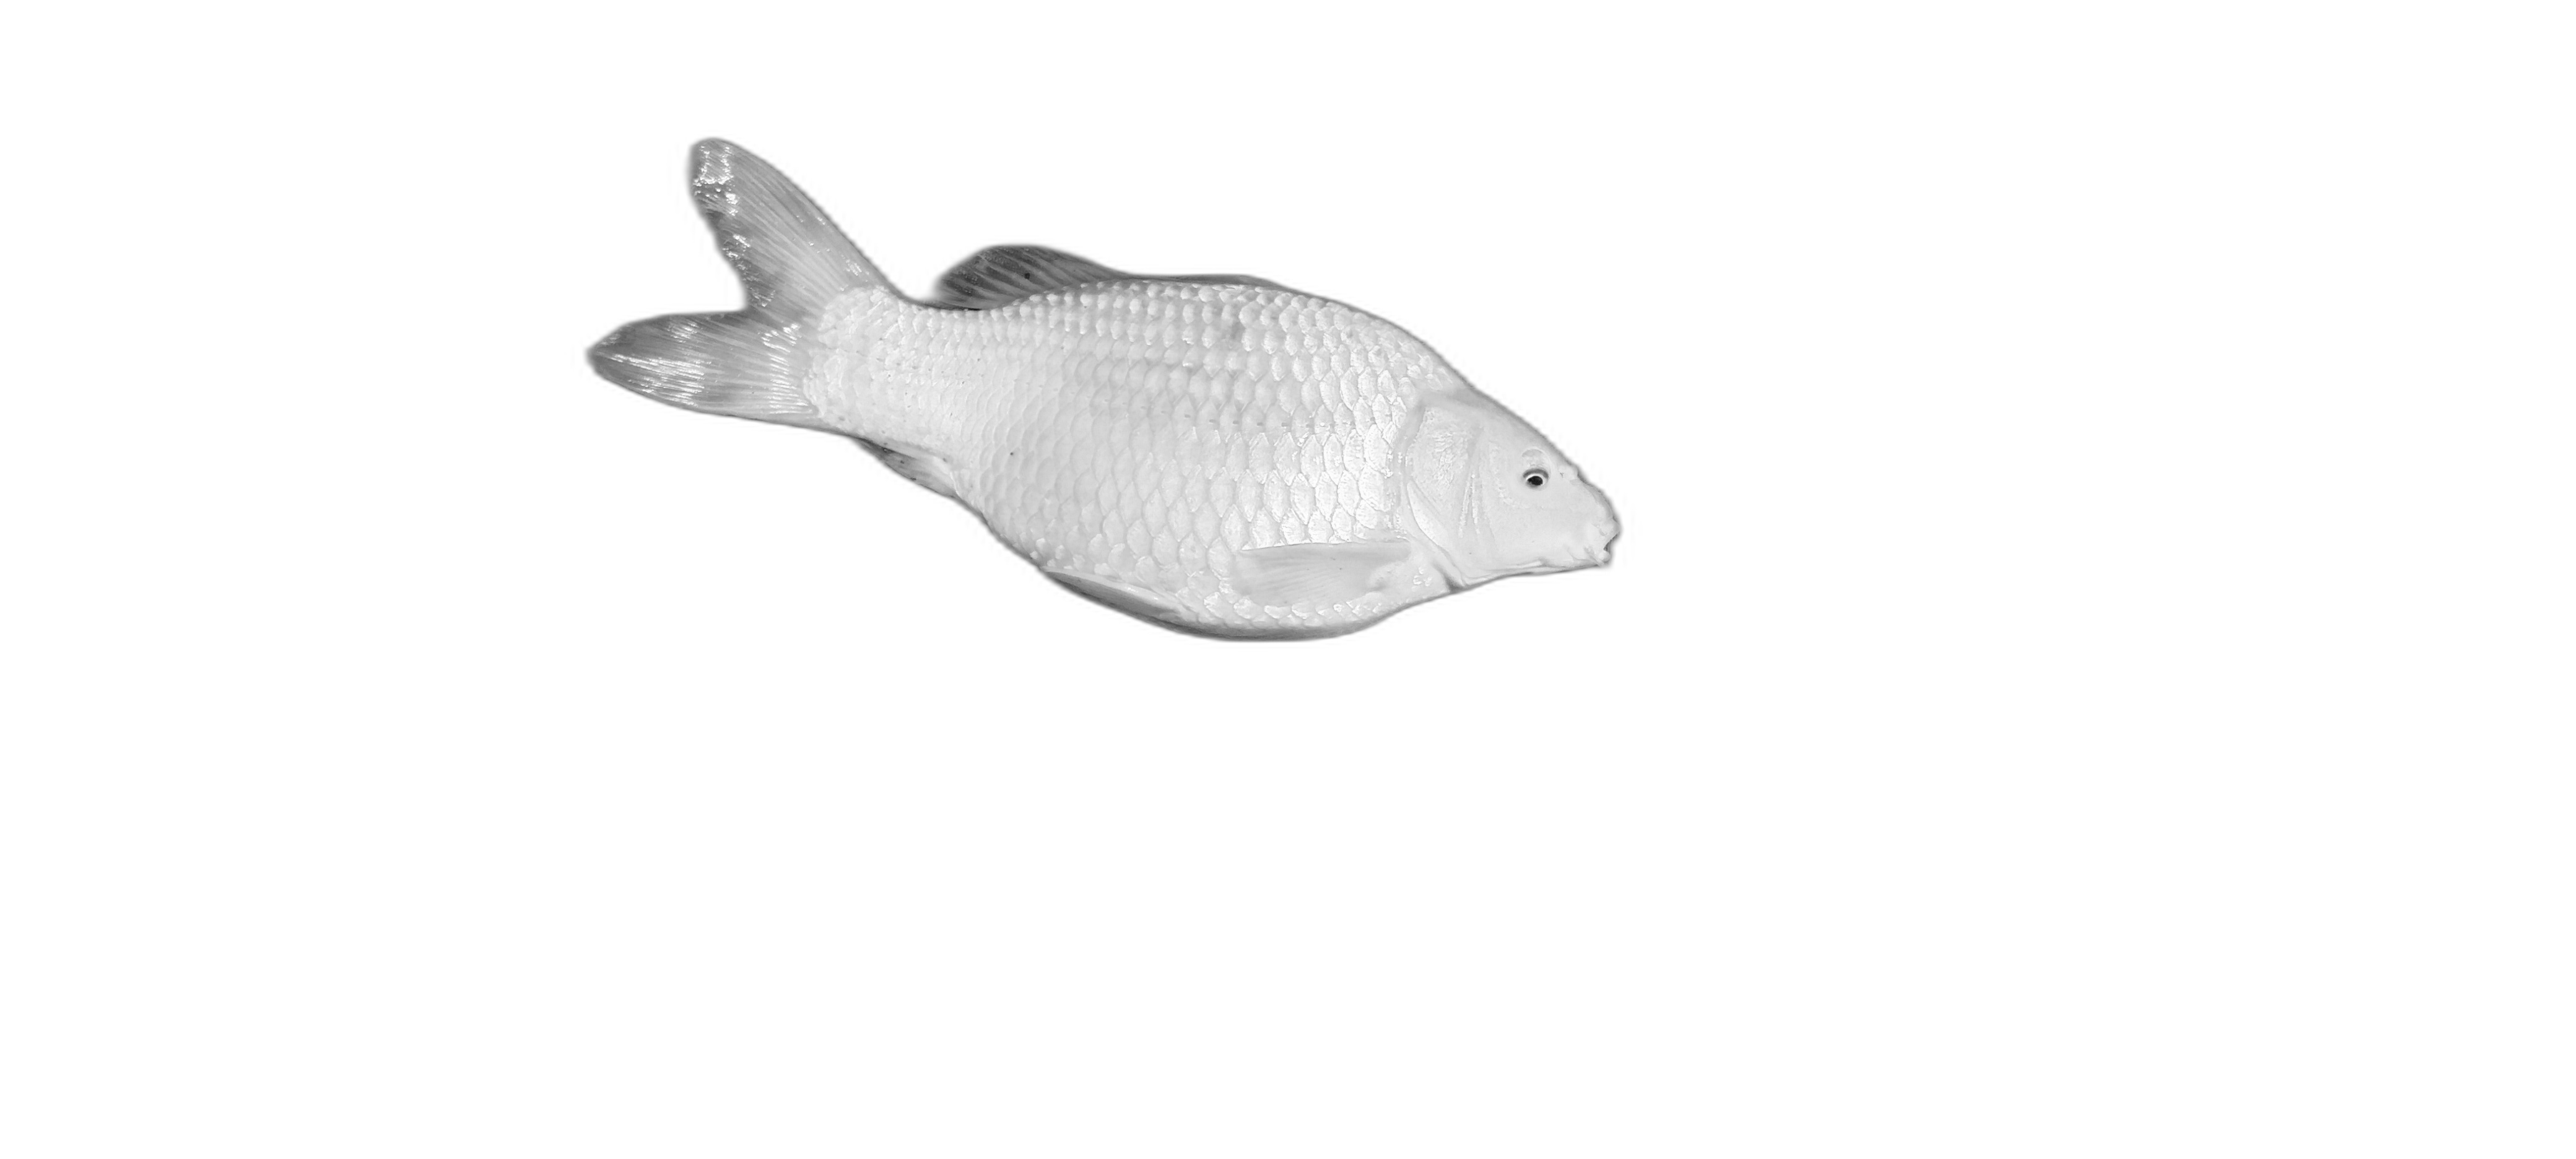
\includegraphics[keepaspectratio, width=4cm]{gambar/IMG_20240121_131125 - Output.jpg}
            \caption{Sebelum Rotasi}
        \end{subfigure}
        \begin{subfigure}{.3\textwidth}
            \centering
            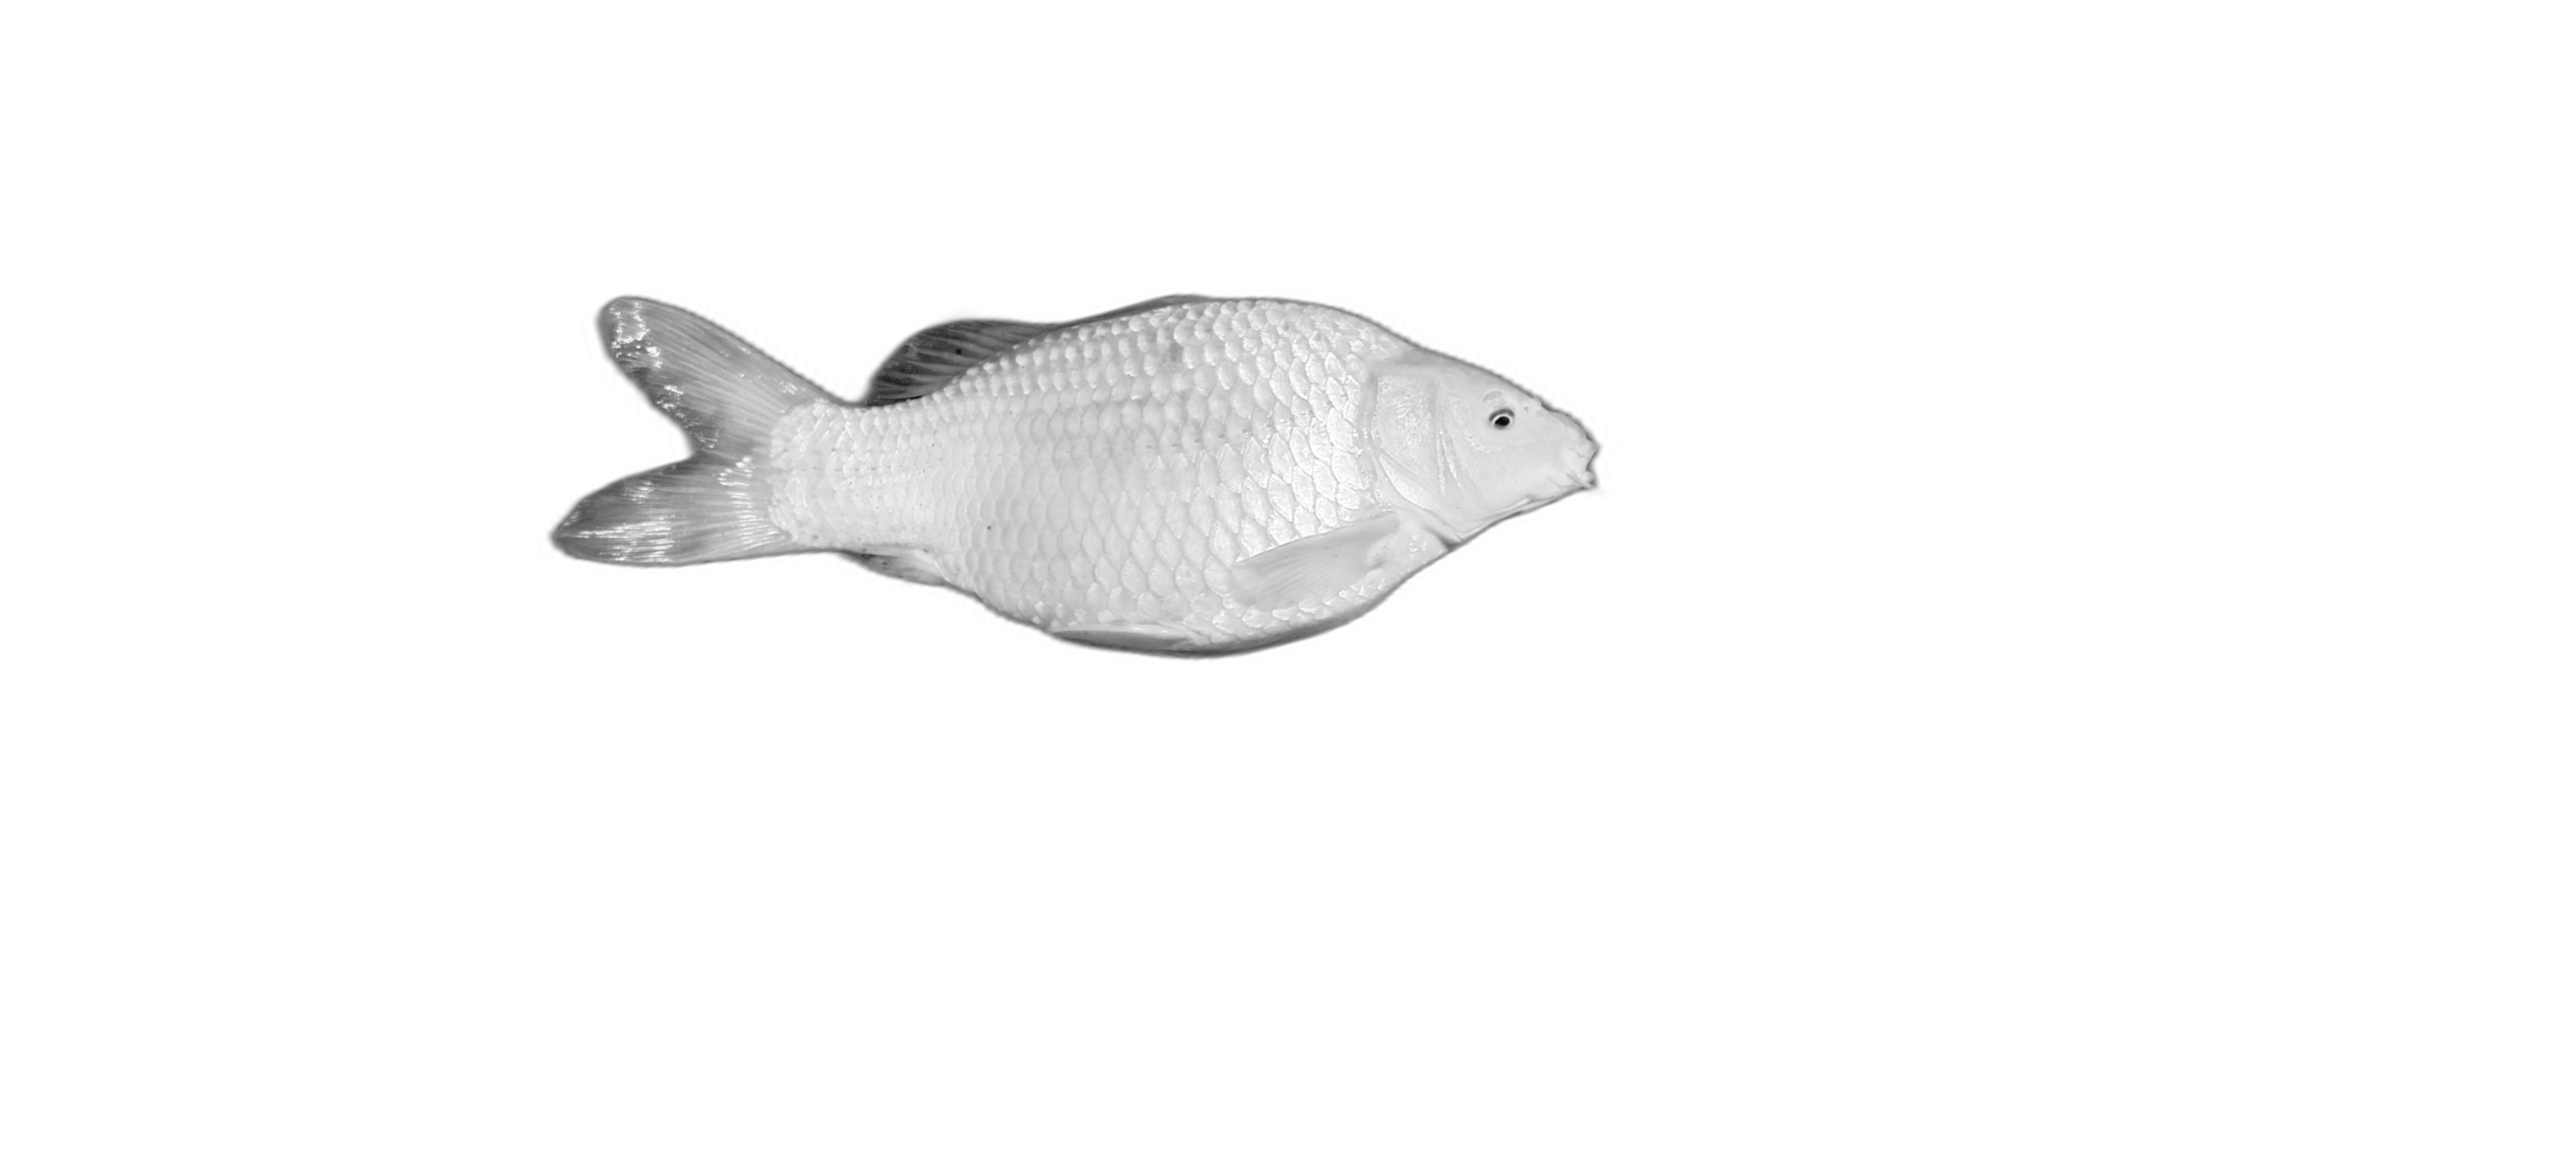
\includegraphics[keepaspectratio, width=4cm]{gambar/IMG_20240121_131125 - rotate.jpg}
            \caption{Setelah Rotasi}
        \end{subfigure}
        \caption{Contoh hasil gambar yang telah dirotasi}\label{fig:rotasi}
    \end{figure}

\subsection{Smoothing Gaussian}

\begin{figure}[H]
    \begin{lstlisting}[language=Python, basicstyle=\tiny]
        def GaussianSmooth(image):
            if len(image.shape) == 3:  
                image = cv2.cvtColor(image, cv2.COLOR_BGR2GRAY)
            elif len(image.shape) == 2: 
                pass

            blurred_image = cv2.GaussianBlur(image, (3, 3), sigmaX=1)
            # Normalize the image to the range [0, 255]
            blurred_image = cv2.normalize(blurred_image, None, 0, 255, cv2.NORM_MINMAX)

            return blurred_image
    \end{lstlisting}
\end{figure}

\emph{GaussianSmooth()} bertujuan untuk menghaluskan citra dengan menggunakan filter Gaussian. Fungsi ini pertama-tama memeriksa apakah citra memiliki tiga saluran warna (RGB) atau hanya satu saluran (grayscale). Jika citra memiliki tiga saluran, maka akan dikonversi menjadi grayscale menggunakan fungsi \emph{cv2.cvtColor}. Setelah itu, fungsi \emph{cv2.GaussianBlur} digunakan untuk menerapkan filter Gaussian pada citra dengan kernel berukuran 3x3 dan nilai sigmaX sebesar 1. Hasil dari proses ini kemudian dinormalisasi ke rentang [0, 255] menggunakan fungsi \emph{cv2.normalize} untuk memastikan bahwa nilai piksel berada dalam rentang yang valid untuk citra grayscale. 
Setelah semua tahapan pra-processing telah selesai dilakukan, gambar akan disave kedalam folder terpisah dan akan digunakan untuk proses selanjutnya.

% \section{Penghitungan Harris Respon}
\section{Menghitung Gradien}
    Sebelum menjalankan fungsi \emph{Harris Respons}, beberapa fungsi perlu dijalankan terlebih dahulu, yaitu menghitung Gradien pada sumbu X dan Y\@. Berikut \emph{Source Code} yang digunakan untuk menghitung Gradien pada sumbu X dan Y:

\begin{figure}[H]
    \begin{lstlisting}[language=Python, basicstyle=\tiny]
        def Compute_Gradient_X(image):
            kernel_x = np.array([[-1, 0, 1],
                                 [-2, 0, 2],
                                 [-1, 0, 1]], dtype=np.float32)
            gradient_x = cv2.filter2D(image, -1, kernel_x)
            return gradient_x

        def Compute_Gradient_Y(image):
            kernel_y = np.array([[1, 2, 1],
                                 [0, 0, 0],
                                 [-1, -2, -1]], dtype=np.float32)
            gradient_y = cv2.filter2D(image, -1, kernel_y)
            return gradient_y
    \end{lstlisting}
    \caption{\emph{source code}: Untuk menghitung Gradien pada sumbu X dan Y}
\end{figure}

    Fungsi \emph{Compute\_Gradient\_X} dan \emph{Compute\_Gradient\_Y} menggunakan kernel Sobel untuk menghitung gradien pada sumbu X (Horizontal) dan Y (Vertical).
Hasil dari proses gradien menunjukkan bahwa bagian tepi tubuh ikan memiliki perubahan intensitas yang cukup tinggi dibandingkan area lainnya. 
Nilai gradien terbesar umumnya muncul pada bagian kepala, ekor, dan sirip ikan karena area tersebut memiliki perubahan bentuk dan kontras yang lebih signifikan terhadap latar belakang citra.

Selain itu, penggunaan Gaussian smoothing pada tahap sebelumnya membantu mengurangi noise sehingga hasil gradien menjadi lebih stabil. 
Tanpa proses smoothing, noise kecil pada citra dapat menghasilkan perubahan intensitas palsu yang berpotensi menyebabkan munculnya titik sudut yang tidak sesuai pada proses Harris-Corner Detection.

\section{Auto Korelasi}
  Proses auto korelasi dilakukan dengan mengkalikan hasil dari gradien dengan gaussian blur. Proses ini bertujuan untuk mengukur seberapa besarnya perubahan intensitas,~berikut \emph{Source Code} yang digunakan untuk menghitung auto korelasi:
\begin{figure}[H]
    \begin{lstlisting}[language=Python, basicstyle=\tiny]
        def AutoCorrelation(gradient_x, gradient_y):
            Ixx = cv2.GaussianBlur(gradient_x ** 2, (3, 3), sigmaX=1)
            Ixy = cv2.GaussianBlur(gradient_x * gradient_y, (3, 3), sigmaX=1)
            Iyy = cv2.GaussianBlur(gradient_y ** 2, (3, 3), sigmaX=1)
            return Ixx, Ixy, Iyy
    \end{lstlisting}
    \caption{\emph{source code}: Untuk menghitung auto korelasi}
\end{figure}

Pada tahap ini dihasilkan tiga komponen utama, yaitu:
\begin{itemize}
    \item \emph{Ixx} yang representasi dari perubahan intensitas pada sumbu X\@.
    \item \emph{Ixy} yang representasi dari korelasi perubahan intensitas antara sumbu X dan Y\@.
    \item \emph{Iyy} yang representasi dari perubahan intensitas pada sumbu Y\@.
\end{itemize}

Nilai-nilai tersebut kemudian digunakan untuk membentuk matriks auto korelasi $M$ pada setiap piksel citra. Matriks ini digunakan sebagai dasar dalam menghitung nilai respon Harris pada tahap berikutnya.
Area yang memiliki perubahan intensitas tinggi pada dua arah sekaligus akan menghasilkan nilai auto korelasi yang besar. Kondisi ini umumnya terjadi pada bagian sudut objek ikan, seperti ujung kepala dan ekor. 
Sebaliknya, area tubuh ikan yang relatif datar akan menghasilkan perubahan intensitas yang lebih kecil sehingga nilai auto korelasi juga menjadi lebih rendah.

\section{Harris Respon}
    Setelah matriks auto korelasi (\emph{second moment matrix}) diperoleh, tahap selanjutnya adalah menghitung nilai Harris response. 
Tahapan ini bertujuan untuk menentukan apakah suatu piksel pada citra merupakan titik sudut (\emph{corner}), tepi (\emph{edge}), atau area datar (\emph{flat area}).

\begin{figure}[H]
    \begin{lstlisting}[language=Python, basicstyle=\tiny]
        def Harris(Ixx, Ixy, Iyy, k=0.04):
            det = Ixx * Iyy - Ixy ** 2
            trace = Ixx + Iyy
            R = det - k * (trace ** 2)
            return R
    \end{lstlisting}
    \caption{\emph{source code}: Untuk menghitung Harris Respon}
\end{figure}

Pada penelitian ini, nilai konstanta empiris $k$ yang digunakan adalah sebesar 0.04. 
Nilai tersebut digunakan untuk mengontrol sensitivitas deteksi sudut pada citra. 
Nilai $k$ yang terlalu kecil dapat menyebabkan banyak titik tepi terdeteksi sebagai sudut, sedangkan nilai yang terlalu besar dapat menyebabkan beberapa sudut penting tidak terdeteksi.

Hasil perhitungan Harris response menghasilkan nilai respon pada setiap piksel citra. Nilai respon yang besar dan positif menunjukkan bahwa piksel tersebut memiliki perubahan intensitas yang signifikan pada dua arah sekaligus, sehingga berpotensi menjadi titik sudut (\emph{corner}). 
Sebaliknya, nilai respon yang kecil atau bernilai negatif menunjukkan bahwa area tersebut cenderung merupakan tepi (\emph{edge}) atau area datar (\emph{flat area}).

Pada objek ikan, nilai respon Harris terbesar umumnya muncul pada bagian kepala, ekor, dan beberapa bagian sirip ikan. 
Hal ini terjadi karena area tersebut memiliki perubahan bentuk yang cukup tajam dibandingkan bagian tubuh ikan lainnya. 
Sementara itu, bagian tengah tubuh ikan cenderung menghasilkan nilai respon yang lebih rendah karena perubahan intensitasnya relatif lebih stabil.

Hasil Harris response pada tahap ini masih mengandung cukup banyak kandidat titik sudut, termasuk beberapa titik yang muncul akibat noise atau perubahan intensitas kecil pada tubuh ikan. 
Oleh karena itu, diperlukan proses thresholding dan \emph{Non-Maximum Suppression} (NMS) pada tahap berikutnya untuk menyaring titik sudut sehingga hanya titik sudut paling signifikan yang dipertahankan.

\begin{figure}[H]
    \centering
    \begin{subfigure}{.3\textwidth}
        \centering
        \includegraphics[keepaspectratio, width=4cm]{gambar/ikan_mas_1_Harris.jpg}
        \caption{Ikan Mas}
    \end{subfigure}
    \begin{subfigure}{.3\textwidth}
        \centering
        \includegraphics[keepaspectratio, width=4cm]{gambar/ikan_lele_induk_1_Harris.jpg}
        \caption{Ikan lele}
    \end{subfigure} 
    \begin{subfigure}{.3\textwidth}
        \centering
        \includegraphics[keepaspectratio, width=4cm]{gambar/ikan_nila_induk_1_Harris.jpg}
        \caption{Ikan Nila Merah}
    \end{subfigure}
    \caption{Contoh hasil gambar yang telah dilakukan Harris Respon}\label{fig:harris_respon}
\end{figure}

\section{NMS dan thresholding}
Setelah nilai Harris response diperoleh, tahap selanjutnya adalah melakukan proses thresholding dan \emph{Non-Maximum Suppression} (NMS). 
Tahapan ini bertujuan untuk menyaring kandidat titik sudut sehingga hanya titik sudut paling signifikan yang dipertahankan untuk proses selanjutnya.

Pada hasil awal Harris response, masih terdapat banyak piksel yang memiliki nilai respon tinggi, termasuk beberapa titik yang muncul akibat noise, tekstur kecil, atau perubahan intensitas yang tidak terlalu penting. 
Oleh karena itu, diperlukan proses penyaringan agar sistem hanya memilih titik sudut yang benar-benar merepresentasikan bentuk objek ikan.

Tahap pertama adalah thresholding. Proses ini dilakukan dengan menggunakan fungsi \emph{thresholding} terhadap nilai Harris response. 
Piksel dengan nilai respon lebih besar dari nilai ambang akan dipertahankan sebagai kandidat sudut, sedangkan piksel dengan nilai respon di bawah ambang akan diabaikan.

 \begin{figure}[H]
    \begin{lstlisting}[language=Python, basicstyle=\tiny]
        def thresholding(preprocessed_images, Harris_respon, output_dir="Output"):
            os.makedirs(output_dir, exist_ok=True)
            all_corners = []

            for idx, (img, r) in enumerate(zip(preprocessed_images, Harris_respon)):
                R_norm = cv2.normalize(r, None, 0, 255, cv2.NORM_MINMAX)
                R_norm = np.uint8(R_norm)

                thresh = 0.01 * r.max()
                dilated = cv2.dilate(r, None)
                nms_mask = (r == dilated) & (r > thresh)
                corners = np.argwhere(nms_mask)
                all_corners.append(corners)
            return all_corners
    \end{lstlisting}
    \caption{\emph{source code}: Untuk melakukan thresholding dan non-maximum suppression}
\end{figure}

Penggunaan threshold membantu mengurangi jumlah piksel yang diproses lebih lanjut sehingga sistem dapat lebih fokus pada area dengan perubahan intensitas yang signifikan. 
Nilai threshold yang terlalu kecil dapat menyebabkan banyak titik sudut palsu (\emph{false corner}) ikut terdeteksi, sedangkan nilai threshold yang terlalu besar dapat menyebabkan beberapa titik sudut penting pada objek ikan tidak terdeteksi.

Setelah proses thresholding, tahap berikutnya adalah \emph{Non-Maximum Suppression} (NMS). Proses NMS dilakukan untuk menghilangkan titik-titik sudut yang saling berdekatan dan hanya mempertahankan titik dengan nilai respon terbesar pada suatu area lokal.

Pada proses ini, nilai \emph{Harris response} akan didilatasi menggunakan fungsi \emph{cv2.dilate} untuk menemukan nilai maksimum dalam suatu area lokal.
kemudian, dibuat sebuah mask yang menunjukan piksel-piksel yang memiliki nilai respon yang sama dengan hasil thresholding. Hasil piksel-piksel tersebulah yang akan digunakan untuk menghitung panjang dan estimasi berat ikan pada tahap selanjutnya.  

\begin{figure}[H]
    \centering
    \begin{subfigure}{.3\textwidth}
        \centering
        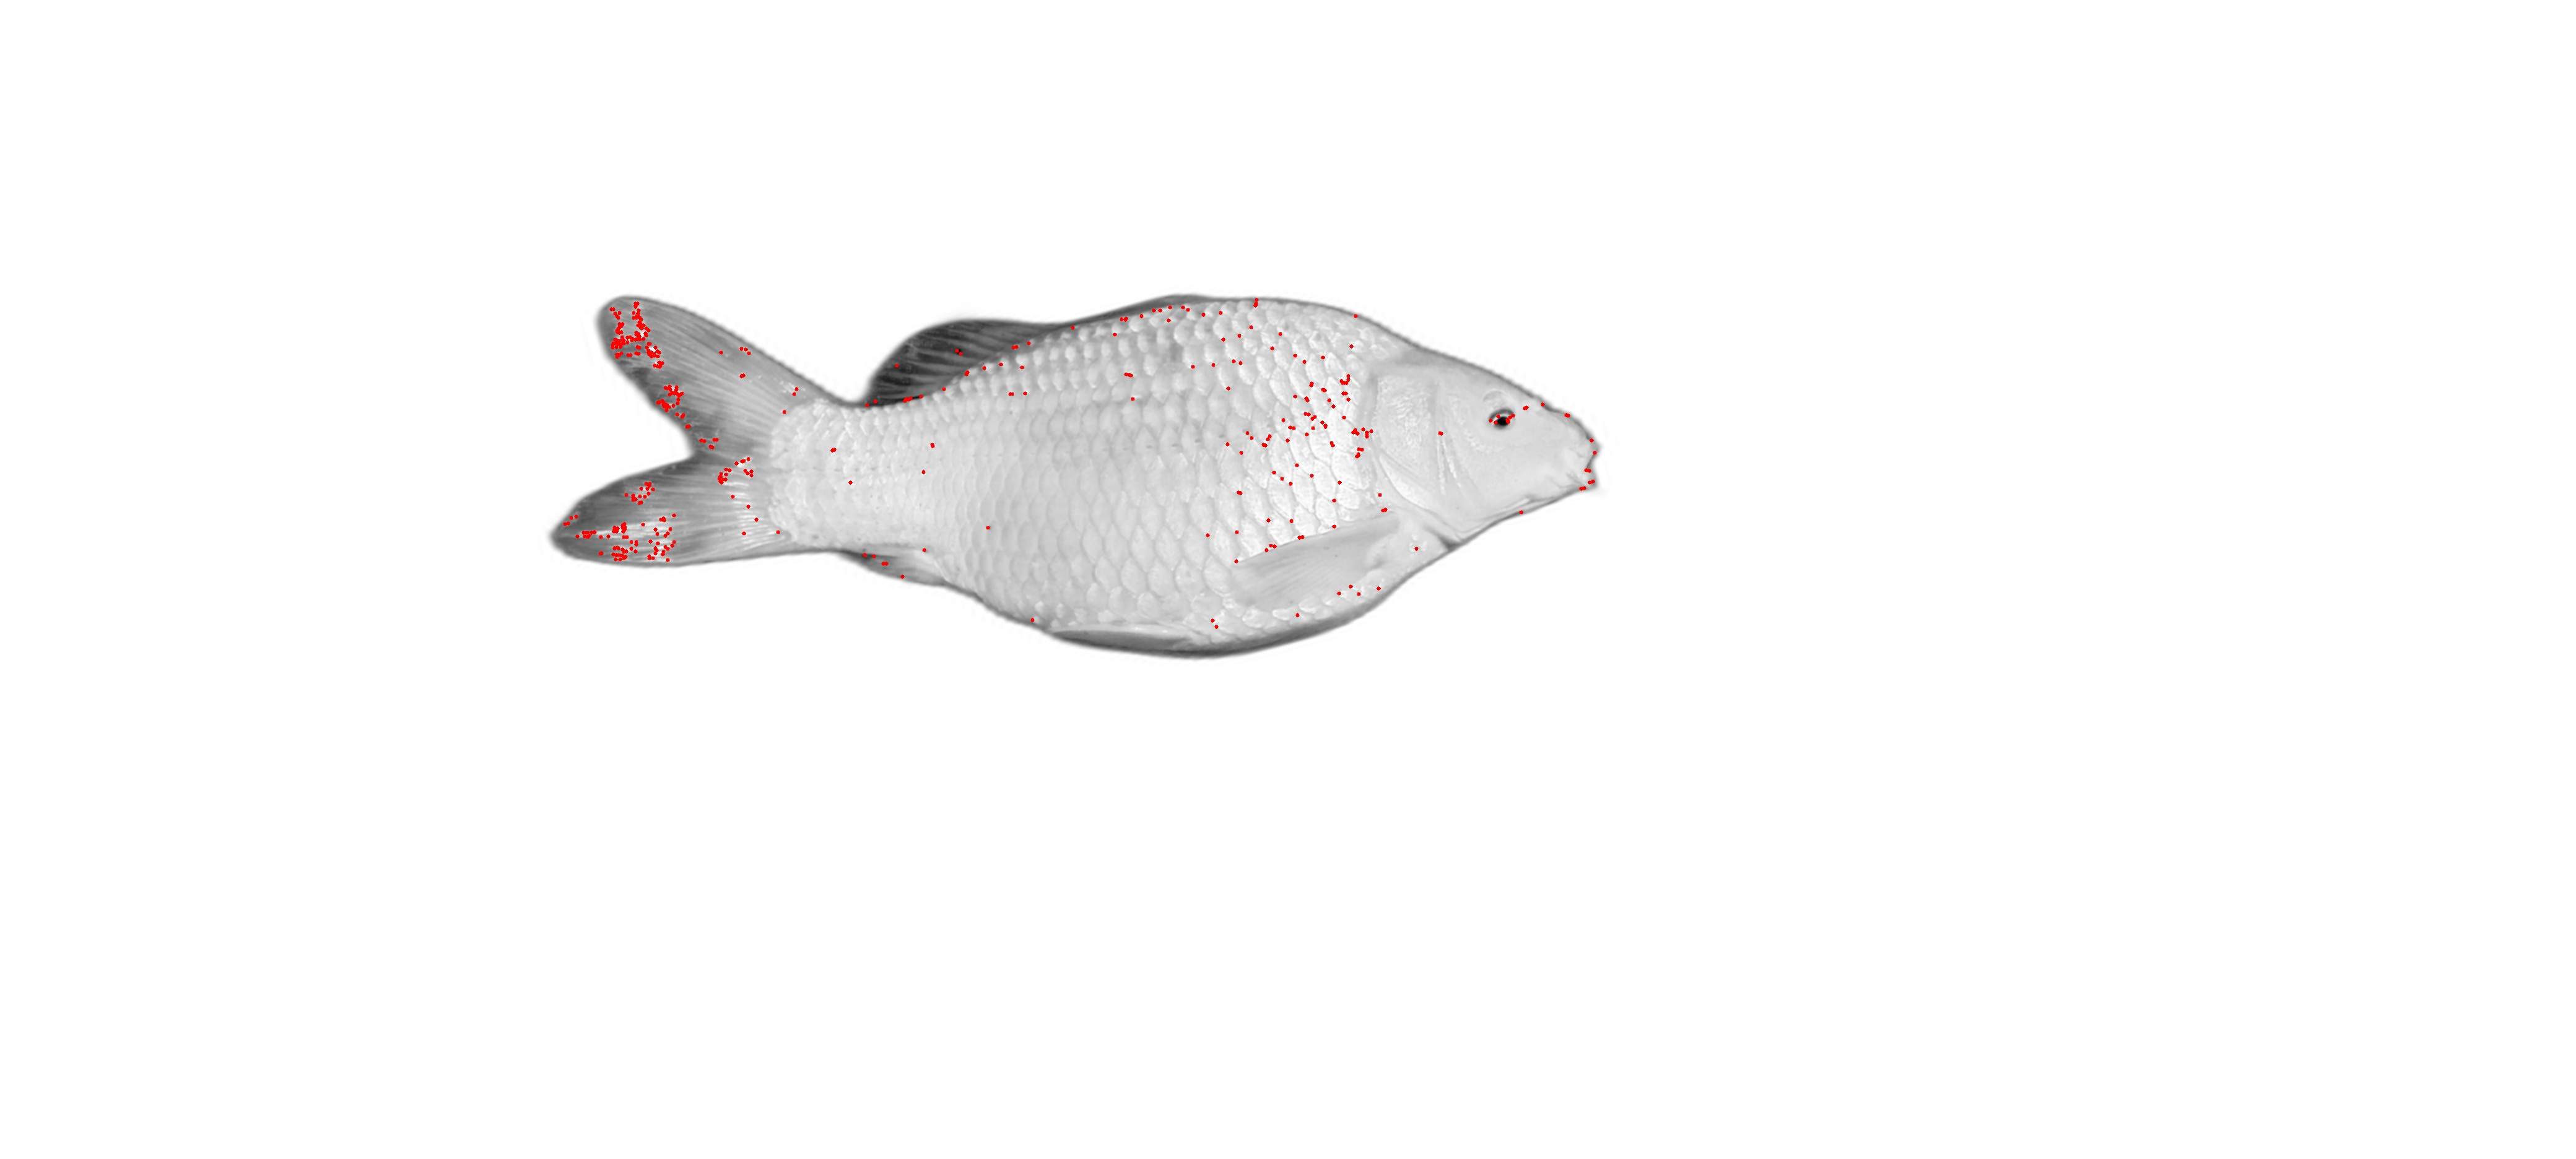
\includegraphics[keepaspectratio, width=4cm]{gambar/ikan_mas_1_NMS.jpg}
        \caption{Ikan Mas}
    \end{subfigure}
    \begin{subfigure}{.3\textwidth}
        \centering
        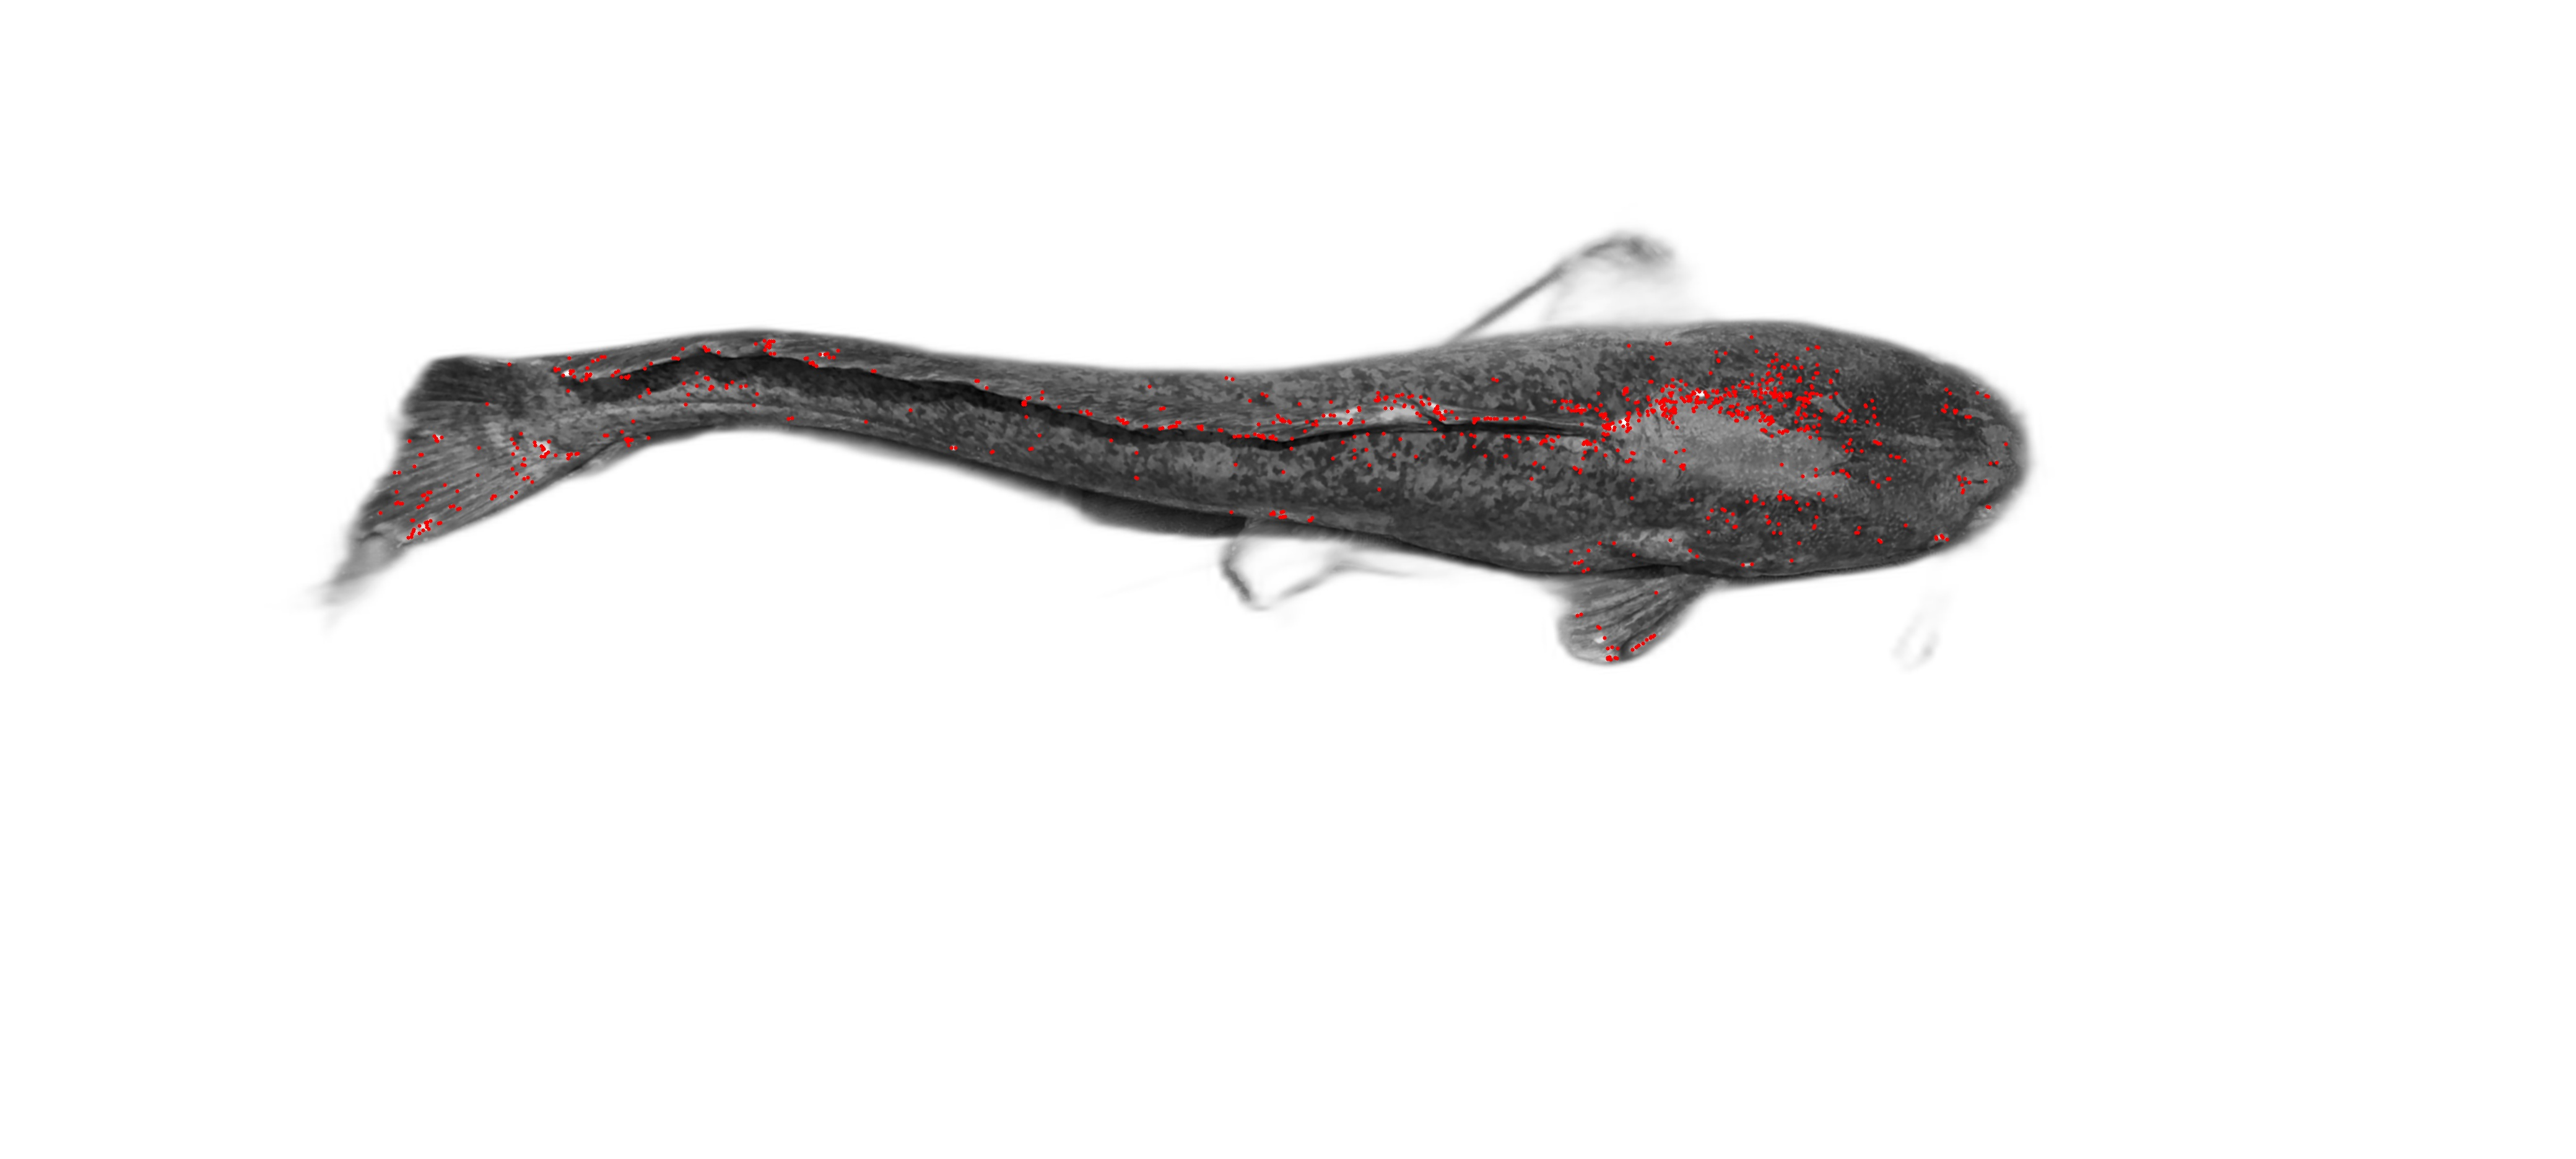
\includegraphics[keepaspectratio, width=4cm]{gambar/ikan_lele_induk_1_NMS.jpg}
        \caption{Ikan lele}
    \end{subfigure} 
    \begin{subfigure}{.3\textwidth}
        \centering
        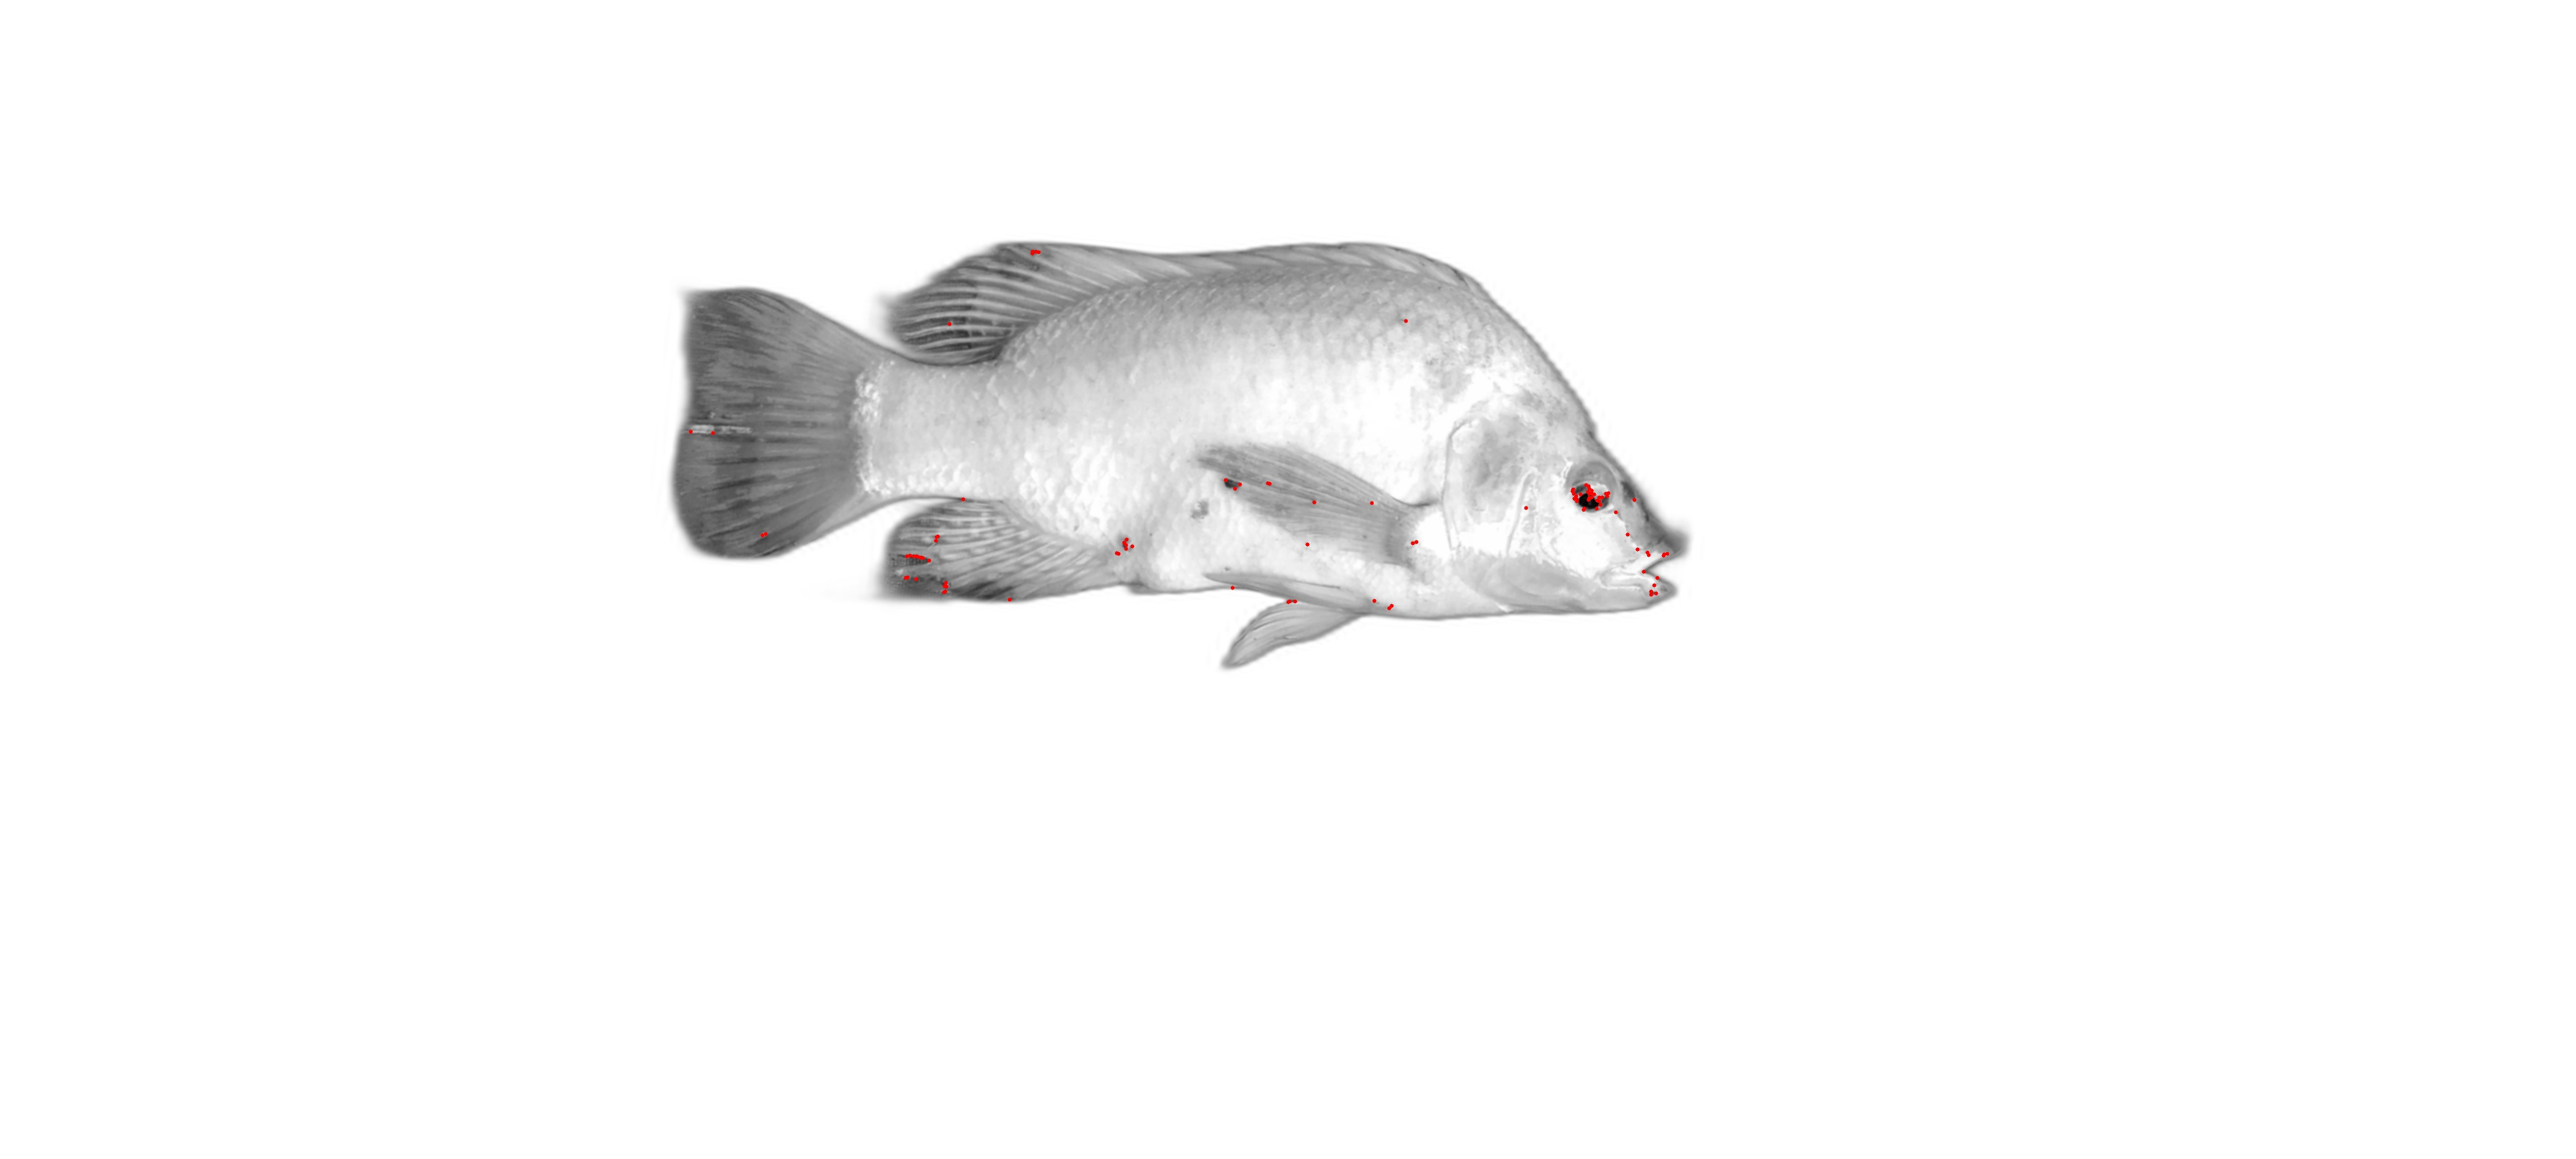
\includegraphics[keepaspectratio, width=4cm]{gambar/ikan_nila_induk_1_NMS.jpg}
        \caption{Ikan Nila Merah}
    \end{subfigure}
    \caption{Contoh hasil gambar yang telah dilakukan thresholding dan NMS}\label{fig:corner}
\end{figure}

\section{Menghitung Panjang dan Berat}
\subsection{Bounding Box}
    Setelah proses thresholding dan Non-Maximum Suppression (NMS) selesai dilakukan, sistem memperoleh kumpulan titik sudut utama (\emph{corner points}) pada objek ikan. 
Titik-titik sudut tersebut kemudian digunakan untuk membentuk bounding box sebagai dasar dalam proses pengukuran panjang dan lebar ikan.
Pemilihan titik sudut untuk bounding box dilakukan dengan menggunakan \emph{Source Code} berikut:
\begin{figure}[H]
    \begin{lstlisting}[language=Python, basicstyle=\tiny]
        def bounding_box(corners):
            if len(corners) == 0:
                return None

            x_min = np.min(corners[:, 1])
            x_max = np.max(corners[:, 1])
            y_min = np.min(corners[:, 0])
            y_max = np.max(corners[:, 0])

            return (x_min, y_min), (x_max, y_max)
    \end{lstlisting}
    \caption{\emph{source code}: Untuk menentukan nilai maksimal dan minimal sumbu x dan y dari titik sudut yang telah didapatkan}
\end{figure}

Pada penelitian ini, bounding box dibentuk menggunakan titik sudut hasil Harris-Corner Detection yang telah melalui proses penyaringan menggunakan thresholding dan NMS\@.
Proses pembentukan bounding box dilakukan dengan mencari:
\begin{itemize}
    \item nilai minimum sumbu-$x$
    \item nilai maksimum sumbu-$x$
    \item nilai minimum sumbu-$y$
    \item nilai maksimum sumbu-$y$
\end{itemize}

Koordinat tersebut digunakan untuk membentuk kotak yang mencakup seluruh tubuh ikan pada citra. 
Panjang dan lebar objek kemudian diperoleh berdasarkan selisih koordinat maksimum dan minimum pada masing-masing sumbu.
Hasil bounding box umumnya mampu mengikuti bentuk tubuh ikan dengan cukup baik, terutama pada citra yang memiliki orientasi horizontal dan hasil segmentasi yang bersih. 
Titik sudut pada bagian kepala dan ekor ikan menjadi acuan utama dalam menentukan panjang objek.
Namun, terdapat beberapa kondisi yang dapat mempengaruhi akurasi bounding box, seperti:
\begin{itemize}
    \item Posisi tubuh ikan yang melengkung.
    \item Titik sudut palsu (\emph{false corner}) akibat noise.
    \item Bagian tubuh ikan yang tidak terdeteksi dengan sempurna.
    \item Bentuk tubuh ikan yang tidak simetris.
\end{itemize}

\begin{figure}[H]
        \centering
    \begin{subfigure}{.3\textwidth}
        \centering
        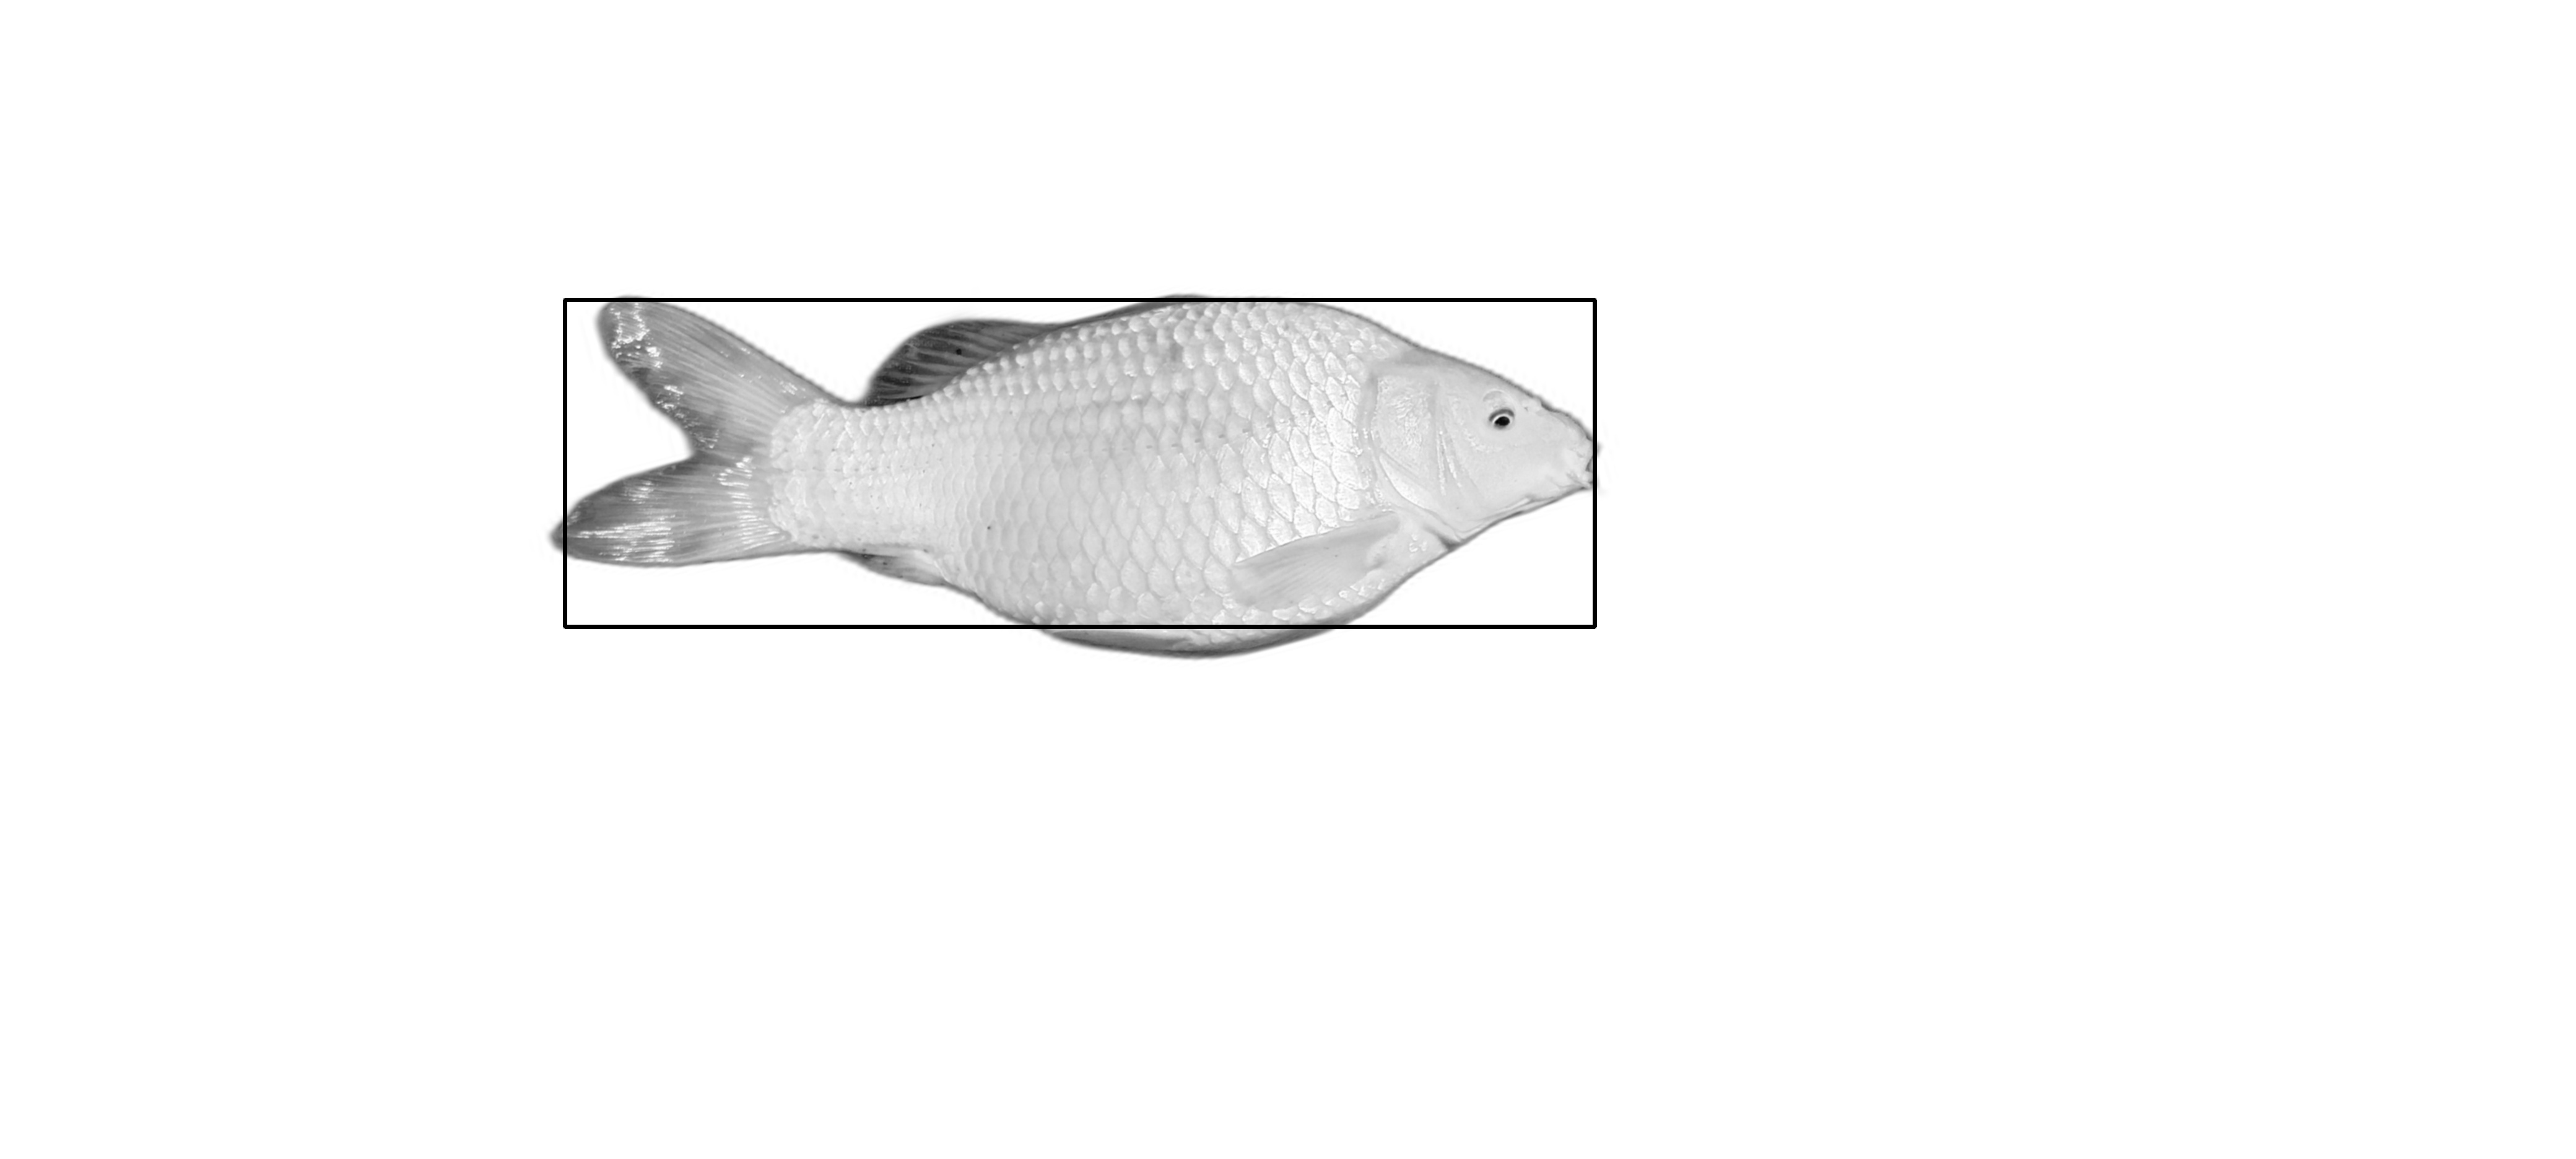
\includegraphics[keepaspectratio, width=4.2cm]{gambar/ikan_mas_1 - Box.jpg}
        \caption{Ikan Mas}
    \end{subfigure}
    \begin{subfigure}{.3\textwidth}
        \centering
        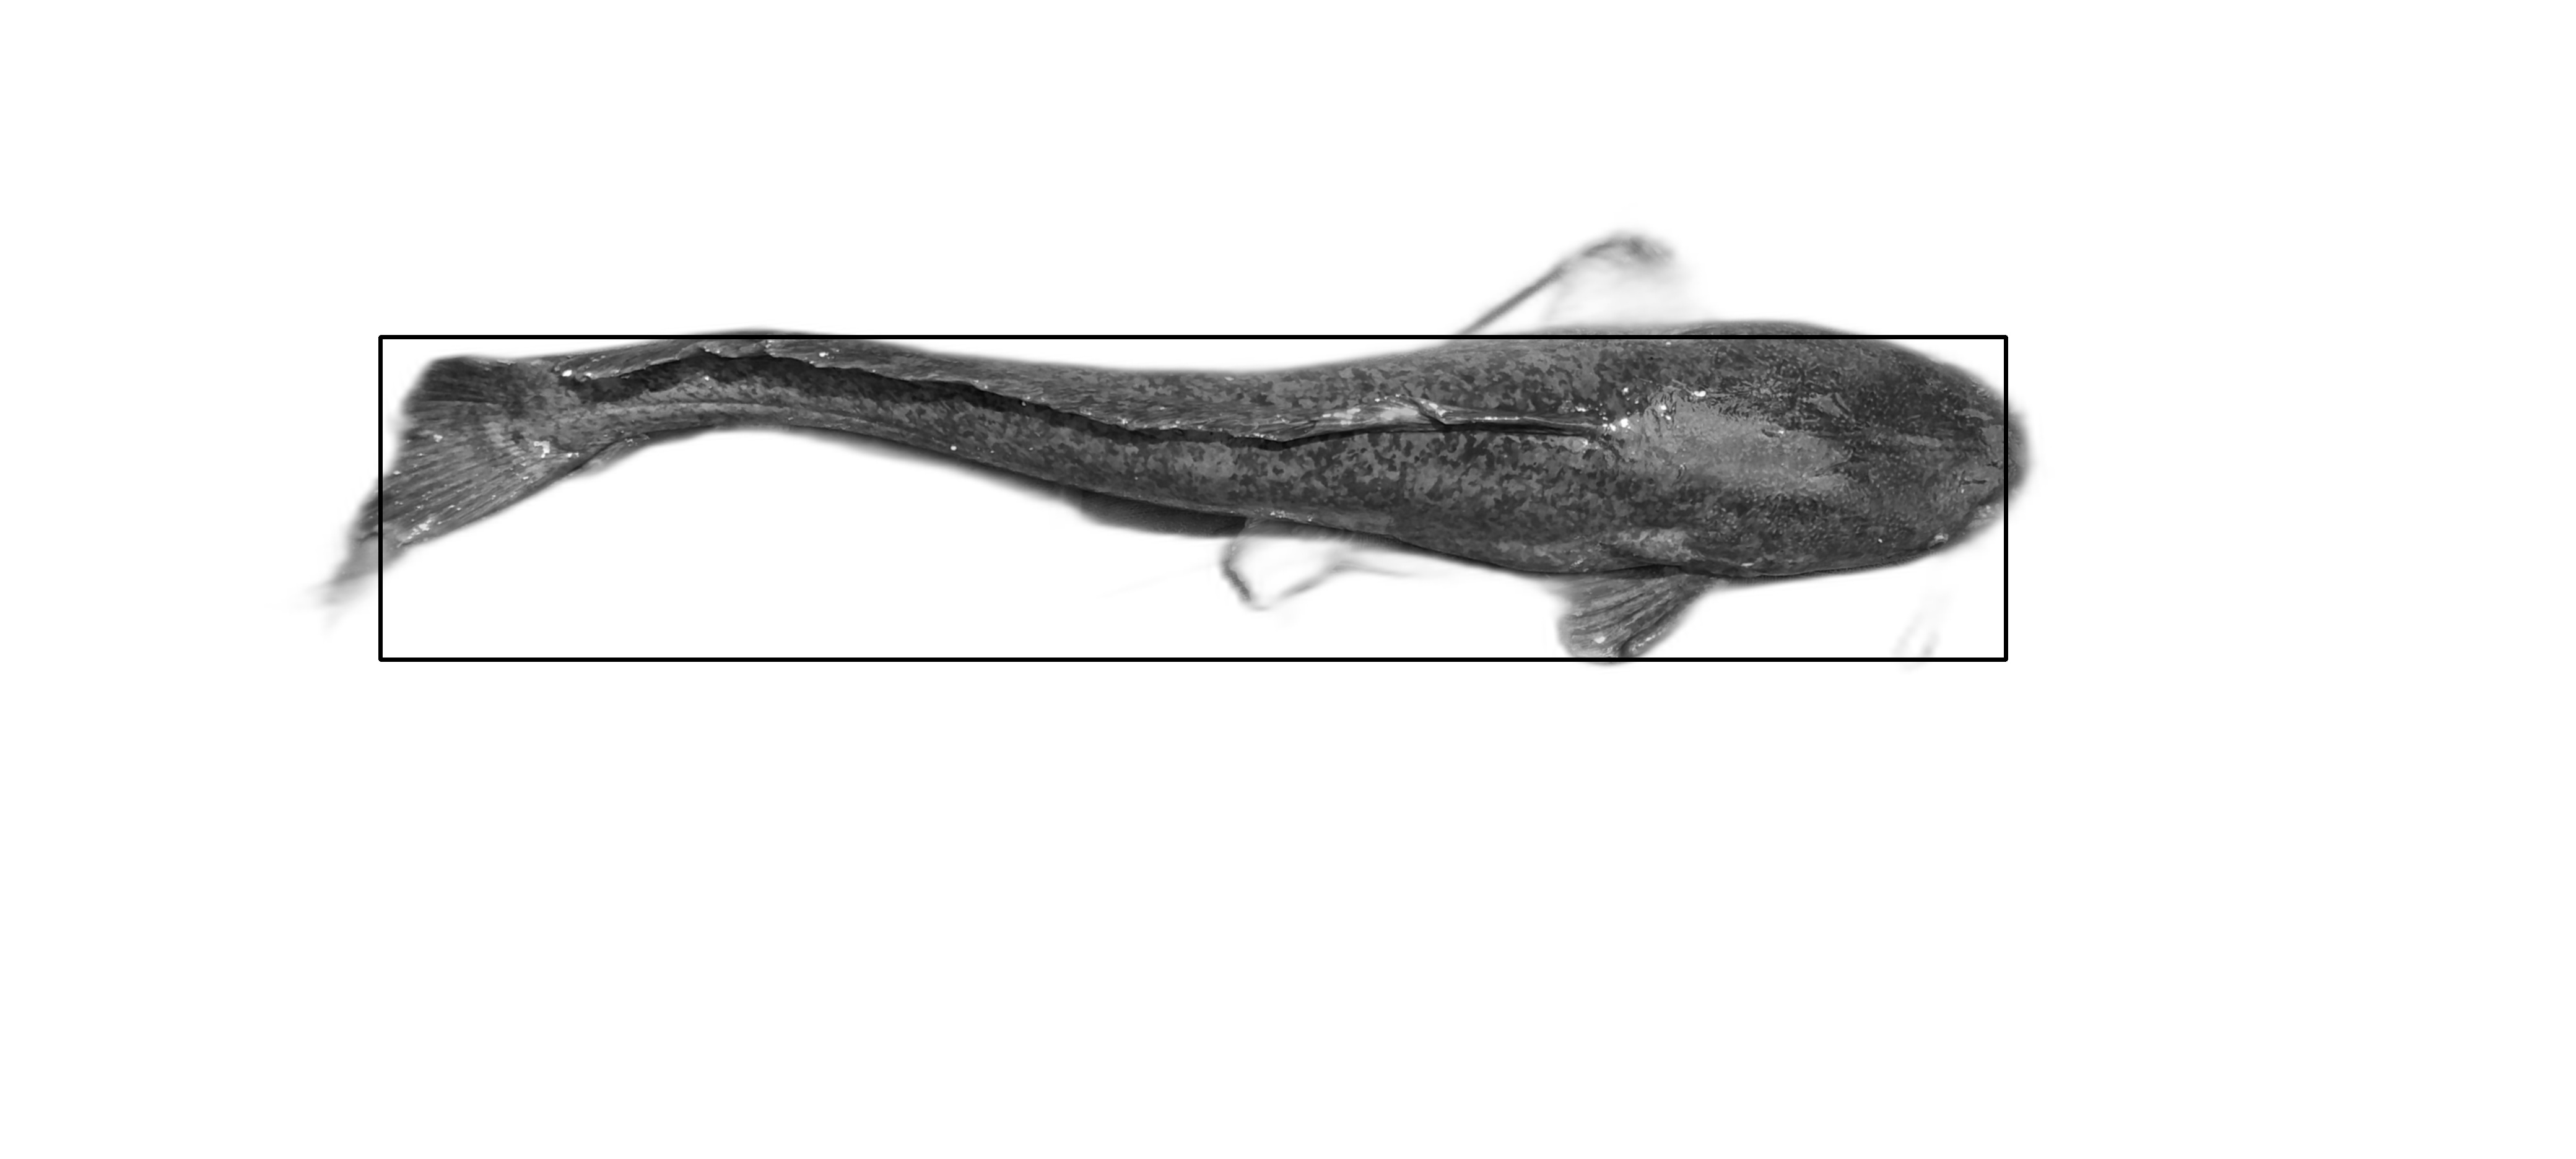
\includegraphics[keepaspectratio, width=4.2cm]{gambar/ikan_lele_1 - Box.jpg}
        \caption{Ikan lele}
    \end{subfigure} 
    \begin{subfigure}{.3\textwidth}
        \centering
        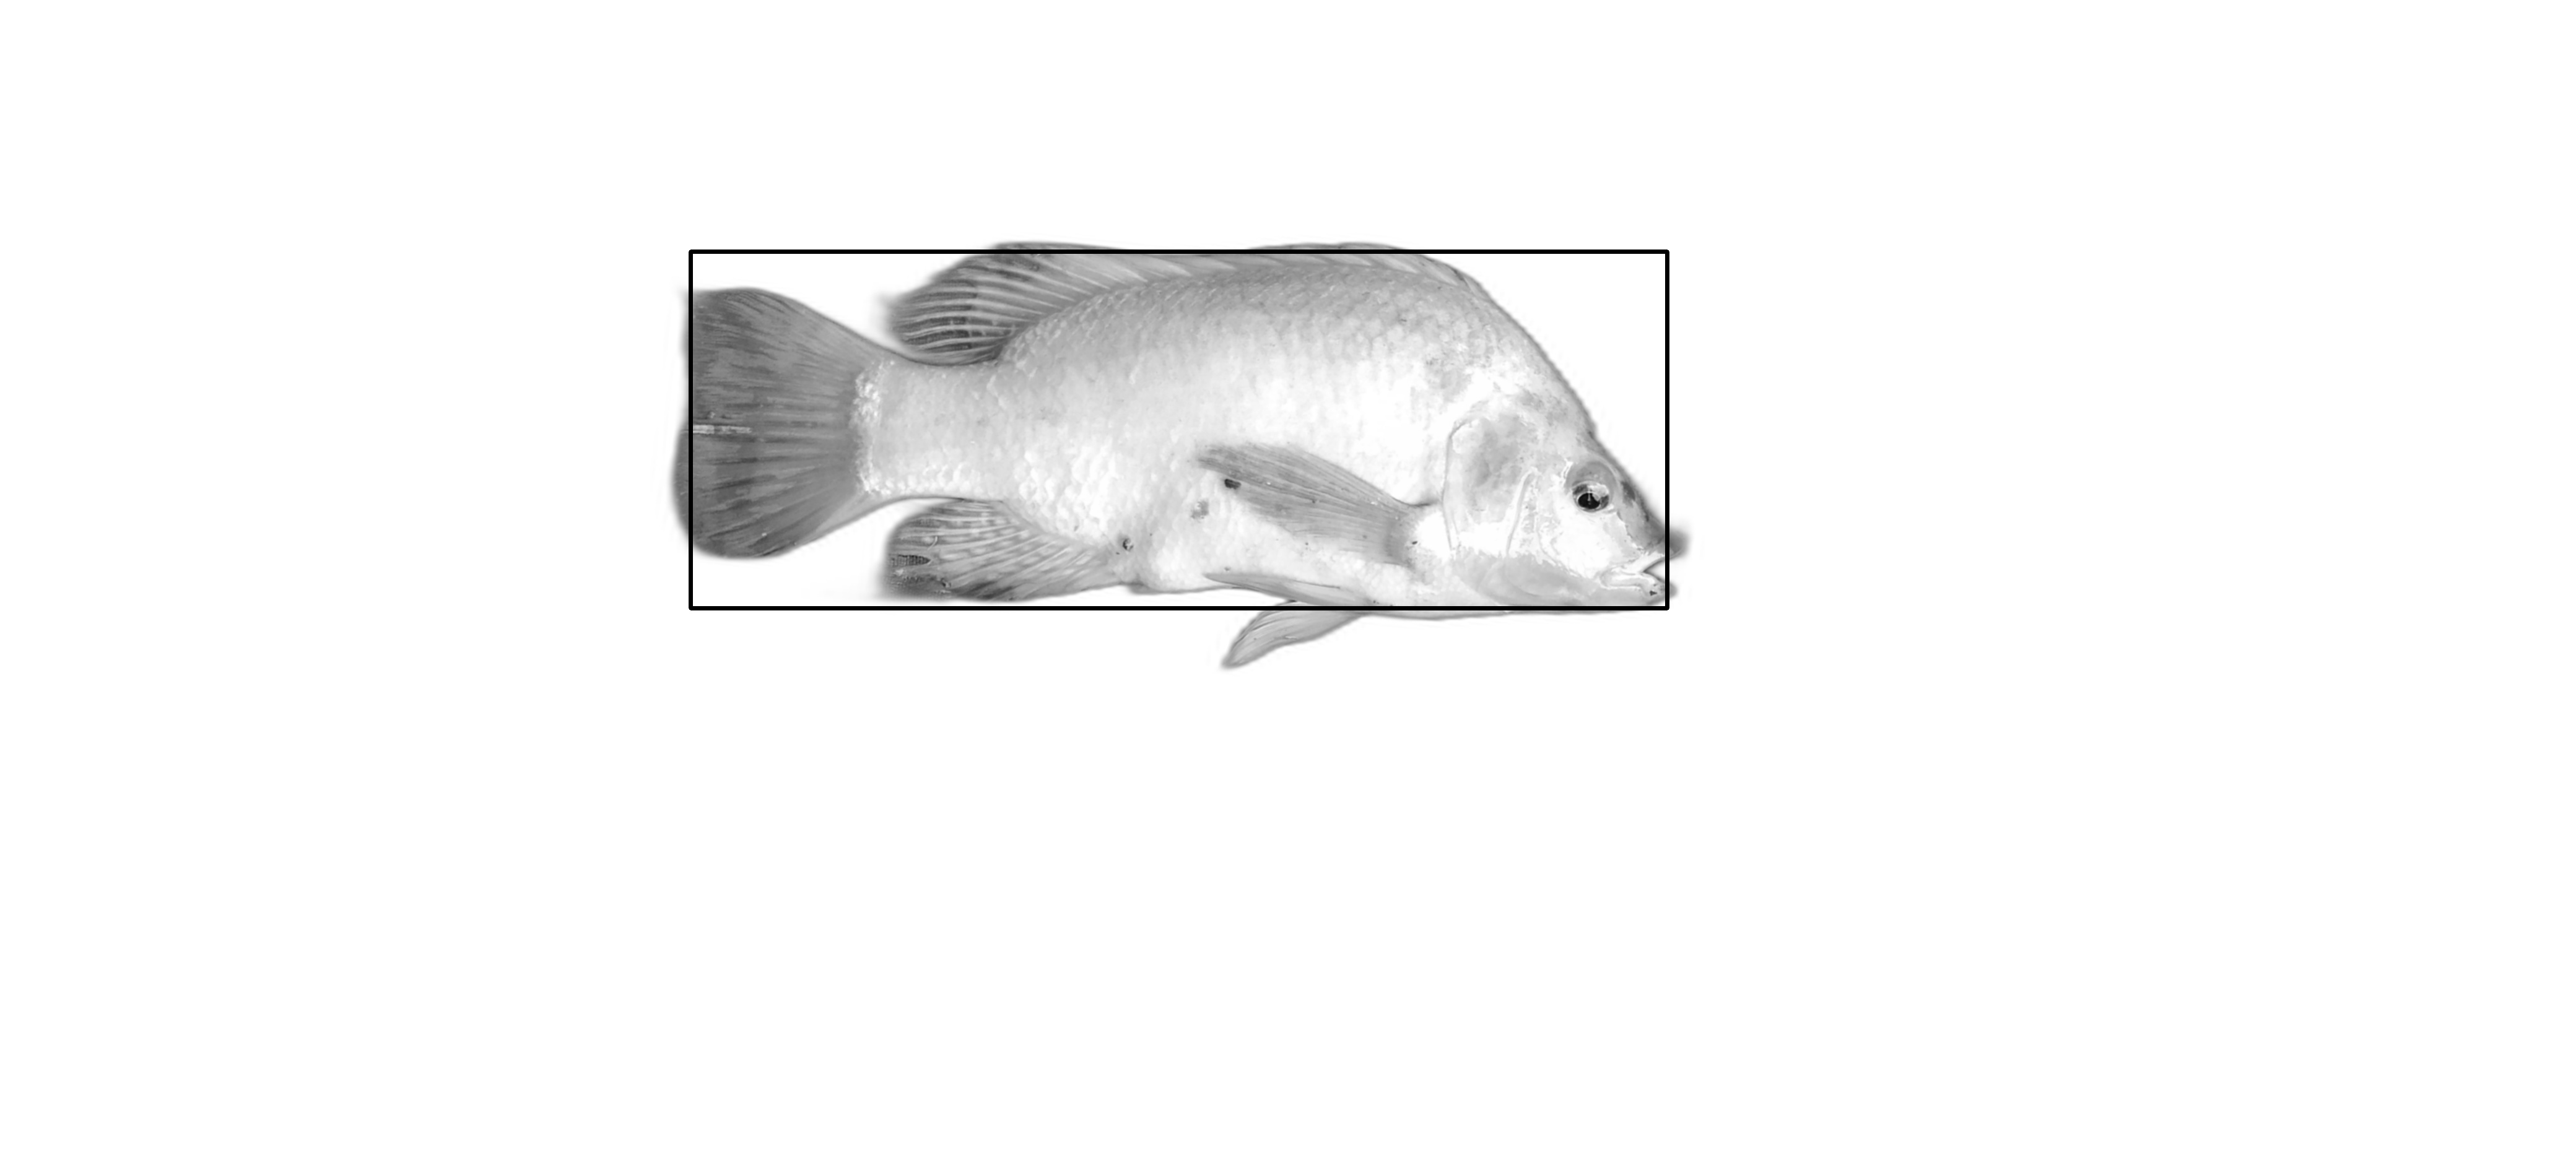
\includegraphics[keepaspectratio, width=4.2cm]{gambar/ikan_nila_1 - Box.jpg}
        \caption{Ikan Nila}
    \end{subfigure}
    \caption{Contoh hasil gambar yang telah diberi bounding box}\label{fig:box}
\end{figure}

Kondisi tersebut dapat menyebabkan ukuran bounding box menjadi terlalu besar atau terlalu kecil sehingga mempengaruhi hasil pengukuran panjang ikan pada tahap berikutnya.

Meskipun demikian, penggunaan bounding box pada penelitian ini cukup efektif untuk merepresentasikan dimensi utama tubuh ikan dan digunakan sebagai dasar dalam proses penghitungan panjang serta estimasi berat ikan.


\subsection{Menghitung Panjang}
    Nilai yang didapatkan dari hasil bounding box akan digunakan untuk menghitung panjang, lebar, dan keliling ikan. Berikut \emph{Source Code} yang digunakan untuk menghitung ukuran ikan:
\begin{figure}[H]
    \begin{lstlisting}[language=Python, basicstyle=\tiny]
        def calculate_size(corners):
            sk = 0.0138  # Skala konversi piksel ke sentimeter
            if corners is None:
                return None

            (x_min, y_min), (x_max, y_max) = bounding_box(corners)
            length_px = abs(x_max - x_min)
            width_px = abs(y_max - y_min)
            
            length = length_px * sk
            width = width_px * sk
            keliling = 2 * (length + width)

            return length, width, keliling
    \end{lstlisting}
    \caption{\emph{source code}: Untuk menghitung panjang, lebar, dan keliling ikan}
\end{figure}

Nilai \emph{sk} merupakan skala konversi dari piksel ke sentimeter yang didapatkan dengan membandingkan ukuran sebuah koin dengan ukuran koin pada gambar.
Gambar koin tersebut diambil dengan menggunakan kamera dan tinggi pengambilan gambar yang sama dengan saat pengambilan gambar ikan.

\subsection{Memproyeksi Perspectif}
    Setelah panjang dan lebar ikan didapatkan, langkah selanjutnya adalah dengan melakukan proyeksi perspektif untuk mengoreksi distorsi yang terjadi pada gambar akibat sudut pengambilan gambar yang tidak sejajar dengan objek. Berikut \emph{Source Code} yang digunakan untuk melakukan proyeksi perspektif:
\begin{figure}[H]
    \begin{lstlisting}[language=Python, basicstyle=\tiny]
        def transform_size(excel_file, sheet_name, folder, panjang_deteksi, lebar_deteksi):
            df = pd.read_excel(excel_file, sheet_name=sheet_name)
            df["nama_file"] = df["nama_file"].astype(str).str.strip().str.lower()
            df = df.set_index('nama_file')

            for files in os.listdir(folder):
                if files.lower().endswith((".jpg", ".png", ".jpeg")):
                    filename = os.path.basename(files)
                    filename = os.path.splitext(filename)[0]
                    filename = filename.lower()
                    # print(filename)
    
                if filename in df.index:
                    panjang_Gt = df.loc[filename, 'panjang']
                    
                    panjang_transformed = panjang_deteksi * (panjang_Gt / panjang_deteksi)
                    lebar_transformed = lebar_deteksi * (panjang_Gt / panjang_deteksi)
                    
                return panjang_transformed, lebar_transformed
    \end{lstlisting}
    \caption{\emph{source code}: Untuk melakukan proyeksi perspektif}
\end{figure}

fungsi \emph{transform\_size} digunakan untuk melakukan proyeksi perspektif dengan menggunakan nilai panjang deteksi yang didapatkan dari hasil perhitungan panjang ikan dan nilai panjang GT yang didapatkan dari tabel referensi. Nilai panjang GT digunakan untuk mengoreksi panjang deteksi sehingga mendapatkan panjang yang lebih akurat. Setelah itu, nilai lebar juga akan dikoreksi dengan menggunakan rasio antara panjang GT dan panjang deteksi.

\subsection{Mengitung Berat}
    Nilai keliling hasil dari fungsi \emph{calculate\_size} akan digunakan untuk menghitung berat ikan. Namun sebelum itu, ikan perlu melalui proses pengecekan jenis ikan, karena berat ikan akan berbeda tergantung jenis ikan. Berikut \emph{Source Code} yang digunakan untuk menghitung berat ikan:
\begin{figure}[H]
    \begin{lstlisting}[language=Python, basicstyle=\tiny]
        def calculate_weight(keliling, filename):
            alm = 2.00
            all_induk = 2.00
            all_pembesar = 1.59
            all_pedaging = 1.07
            aln_induk = 1.29
            aln_kdua  = 1.13
            aln_kbawah = 1.08
            
            Berat = 0
            if "mas" in filename:
                    Berat = alm * luas
            elif "lele" in filename and "induk" in filename:
                    Berat = all_induk * luas
            elif "lele" in filename and "pembesaran" in filename:
                Berat = all_pembesar * luas
            elif "lele" in filename and "pedaging" in filename:
                Berat = all_pedaging * luas
            elif "nila" in filename and "induk" in filename:
                    Berat = aln_induk * luas
            elif "nila" and "kdua" in filename:
                Berat = aln_kdua * luas
            elif "nila" and "kbawah" in filename:
                Berat = aln_kbawah * luas
            else:
                    break
    \end{lstlisting}
    \caption{\emph{source code}: Untuk mengestimasi berat ikan berdasarkan Rumus turunan \emph{Length-Weight Relationship}}
    
\end{figure}

     \emph{akm}, \emph{akl}, dan \emph{akn} merupakan nilai hasil dari rata-rata berat dengan keliling ikan nyata pada setiap jenis ikan. 
Nilai tersebut didapatkan dengan melakukan pengukuran langsung pada ikan nyata dengan menggunakan pita ukur untuk mendapatkan keliling ikan dan timbangan untuk mendapatkan berat ikan. Setelah itu, dilakukan perhitungan rata-rata berat dengan keliling ikan nyata untuk mendapatkan nilai \emph{akm}, \emph{akl}, dan \emph{akn}.

\section{Evaluasi Akurasi}
    Nilai hasil penghitungan panjang, lebar, dan berat ikan akan dibandingkan dengan nilai panjang, lebar, dan berat ikan referensi.
Nilai referensi yang digunakan dapat dilihat pada tabel~\ref{tab:Nilai Referensi}.

Setelah dilakukan evaluasi akurasi terhadap hasil deteksi panjang, lebar, dan estimasi berat ikan, ditemukan bahwa beberapa hasil estimasi berat ikan ada yang kurang, bahkan ada yang melebihi dari nilai referensi-nya. Hasil deteksi panjang, lebar, dan estimasi berat dapat di lihat pada tabel~\ref{tab:Hasil Deteksi} berikut: %Hal ini disebabkan oleh beberapa faktor, yaitu:

% \begin{enumerate}
%     \item Proses penghitungan berat ikan yang menggunakan nilai luas ikan sebagai input, sehingga jika terdapat kesalahan pada proses penghitungan panjang dan lebar ikan, maka akan berpengaruh pada hasil estimasi berat ikan.
%     \item Nilai \emph{sk} yang digunakan untuk mengkonversi piksel ke sentimeter merupakan nilai yang didapatkan dengan membandingkan ukuran sebuah koin dengan ukuran koin pada gambar. Jika terdapat kesalahan dalam pengukuran ukuran koin atau jika ukuran koin pada gambar tidak sesuai dengan ukuran koin yang sebenarnya, maka akan berpengaruh pada hasil konversi piksel ke sentimeter, sehingga dapat menyebabkan kesalahan dalam perhitungan panjang dan lebar ikan.
%     \item Proses proyeksi perspektif yang digunakan untuk mengoreksi distorsi pada gambar juga dapat menyebabkan kesalahan jika nilai panjang GT yang digunakan untuk mengoreksi panjang deteksi tidak akurat atau jika rasio antara panjang GT dan panjang deteksi tidak sesuai.
%     \item Jarak pengambilan gambar atau sudut pengambilan gambar yang tidak konsisten menyebabkan distorsi pada gambar yang tidak dapat sepenuhnya dikoreksi dengan proyeksi perspektif, sehingga menyebabkan kesalahan dalam perhitungan panjang dan lebar ikan.
% \end{enumerate}

% beberapa hasil deteksi dapat dilihat pada tabel~\ref{tab:Hasil Deteksi} berikut:

\begin{longtable}{|c|c|c|c|c|}
        \hline
        No. & Nama File & Panjang (cm) & Lebar (cm) & Berat (g) \\
        \hline
        \endfirsthead
        \multicolumn{5}{c}{{\tablename\ \thetable{} -- continued from previous page}} \\
        \hline
        No. & Nama File & Panjang (cm) & Lebar (cm) & Berat (g) \\
        \hline
        \endhead
        \hline \multicolumn{5}{|r|}{{Continued on next page}} \\ \hline
        \endfoot
        \hline
        \endlastfoot

        1. & ikan\_mas\_1.jpg & 34 & 10 & 680 \\
        \hline
        2. & ikan\_mas\_2.jpg & 29 & 8 & 464 \\
        \hline
        3. & ikan\_mas\_3.jpg & 37 & 10 & 740 \\
        \hline
        4. & ikan\_mas\_4.jpg & 31 &  8 & 496 \\
        \hline
        5. & ikan\_mas\_5.jpg & 24 & 6 & 288 \\
        \hline
        6. & ikan\_mas\_6.jpg & 26 & 8 & 364 \\
        \hline
        7. & ikan\_lele\_Induk\_1.jpg & 52 & 10 & 1040 \\
        \hline
        8. & ikan\_lele\_Induk\_2.jpg & 54 & 11 & 1188 \\
        \hline
        9. & ikan\_lele\_Induk\_3.jpg & 53 & 12 & 1272 \\
        \hline
        10. & ikan\_lele\_Pembesaran\_4.jpg & 39 & 6 & 372 \\
        \hline
        11. & ikan\_lele\_Pembesaran\_5.jpg & 41 & 7 & 456 \\
        \hline
        12. & ikan\_lele\_Pembesaran\_6.jpg & 35 & 7 & 390 \\
        \hline
        13. & ikan\_lele\_Pembesaran\_7.jpg & 35 & 7 & 390 \\
        \hline
        14. & ikan\_lele\_Pedaging\_8.jpg & 28 & 8 & 240 \\
        \hline
        15. & ikan\_lele\_Pedaging\_9.jpg & 27 & 4 & 116 \\
        \hline
        16. & ikan\_lele\_Pedaging\_10.jpg & 27 & 6 & 173 \\
        \hline
        17. & ikan\_lele\_Pedaging\_11.jpg & 25 & 5 & 133 \\
        \hline
        18. & ikan\_lele\_Pedaging\_12.jpg & 20 & 3 & 64 \\
        \hline
        19. & ikan\_lele\_Pedaging\_13.jpg & 27 & 7 & 202 \\
        \hline
        20. & ikan\_nila\_Induk\_1.jpg & 33 & 12 & 511 \\
        \hline
        21. & ikan\_nila\_Induk\_2.jpg & 31 & 11 & 440 \\
        \hline
        22. & ikan\_nila\_Induk\_3.jpg & 28 & 11 & 397 \\
        \hline
        23. & ikan\_nila\_Kdua\_4.jpg & 25 & 10 & 282 \\
        \hline
        24. & ikan\_nila\_Kdua\_5.jpg & 23 & 10 & 260 \\
        \hline
        25. & ikan\_nila\_Kdua\_6.jpg & 24 & 8 & 217 \\
        \hline
        26. & ikan\_nila\_Kdua\_7.jpg & 24 & 9 & 244 \\
        \hline
        27. & ikan\_nila\_Kdua\_8.jpg & 24 & 7 & 190 \\
        \hline
        28. & ikan\_nila\_kbawah\_9.jpg & 19 & 7 & 144 \\
        \hline
        29. & ikan\_nila\_kbawah\_10.jpg & 22 & 13 & 308 \\
        \hline
        30. & ikan\_nila\_kbawah\_11.jpg & 20 & 8 & 172 \\
        \hline
        31. & ikan\_nila\_kbawah\_12.jpg & 19 & 7 & 144 \\
        \hline
        32. & ikan\_nila\_kbawah\_13.jpg & 20 & 7 & 151 \\
        \hline
    \caption{Hasil Deteksi}\label{tab:Hasil Deteksi}
\end{longtable}

Dengan Menggunakan rumus \emph{Mean Absolute Percentage Error} atau MAPE, didapatkan hasil evaluasi akurasi pada table~\ref{tab:MAPE} berikut:

\begin{table}[H]
    \centering
    \begin{tabular}{|c|c|c|c|c|}
        \hline
        No. & Nama File & Panjang (\%) & Lebar (\%) & Berat (\%) \\
        \hline
        1. & ikan\_mas & 100 & 79.11 & 88.79 \\
        \hline
        2. & ikan\_lele & 99.73 & 73.99 & 67.97 \\
        \hline
        3. & ikan\_nila & 100 & 85.26 & 83.96 \\
        \hline
    \end{tabular}
\caption{Rata-Rata MAPE Ikan}\label{tab:MAPE}
\end{table}

Dan pada table~\ref{tab:allEval} adalah hasil keseluruhan evaluasi akurasi :

\begin{table}[H]
    \centering
    \begin{tabular}{|c|c|c|c|c|}
        \hline
        No. & Nama File & Berat (\%) & Panjang (\%) & Lebar (\%) \\
        \hline
        1. & ikan\_mas\_1.jpg & 91.89 & 100 & 71.43 \\
        \hline
        2. & ikan\_mas\_2.jpg & 92.80 & 100 & 66.67 \\
        \hline
        3. & ikan\_mas\_3.jpg & 96.86 & 100 & 83.33 \\
        \hline
        4. & ikan\_mas\_4.jpg & 93.10 & 100 & 80 \\
        \hline
        5. & ikan\_mas\_5.jpg & 74.78 & 100 & 85/71 \\
        \hline
        6. & ikan\_mas\_6.jpg & 83.33 & 100 & 87.5 \\
        \hline

    \end{tabular}
    \end{table}
    \begin{table}[H]
        \centering
        \begin{tabular}{|c|c|c|c|c|}
        \hline
        No. & Nama File & Berat (\%) & Panjang (\%) & Lebar (\%) \\
        \hline
        7. & ikan\_lele\_Induk\_1.jpg & 74.7 & 100 & 75 \\
        \hline
        8. & ikan\_lele\_Induk\_2.jpg & 73.62 & 100 & 77.78 \\
        \hline
        9. & ikan\_lele\_Induk\_3.jpg & 55.45 & 100 & 150 \\
        \hline
        10. & ikan\_lele\_Pembesaran\_4.jpg & 86.51 & 100 & 85.71 \\
        \hline
        11. & ikan\_lele\_Pembesaran\_5.jpg & 99.13 & 100 & 100 \\
        \hline
        12. & ikan\_lele\_Pembesaran\_6.jpg & 88.57 & 100 & 83.33 \\
        \hline
        13. & ikan\_lele\_Pembesaran\_7.jpg & 78.13 & 100 & 83.33 \\
        \hline
        14. & ikan\_lele\_Pedaging\_8.jpg & 128.57 & 100 & 66.67 \\
        \hline
        15. & ikan\_lele\_Pedaging\_9.jpg & 72.5 & 100 & 66.67 \\
        \hline
        16. & ikan\_lele\_Pedaging\_10.jpg & 127 & 100 & 80 \\
        \hline
        17. & ikan\_lele\_Pedaging\_11.jpg & 89.17 & 100 & 83.33 \\
        \hline
        18. & ikan\_lele\_Pedaging\_12.jpg & 29.09 & 100 & 50 \\
        \hline
        19. & ikan\_lele\_Pedaging\_13.jpg & 81.18 & 96.43 & 60 \\
        \hline
        20. & ikan\_nila\_Induk\_1.jpg & 76.27 & 100 & 85.71 \\
        \hline
        21. & ikan\_nila\_Induk\_2.jpg & 97.78 & 100 & 91.67 \\
        \hline
        22. & ikan\_nila\_Induk\_3.jpg & 92.70 & 100 & 100 \\
        \hline
        23. & ikan\_nila\_Kdua\_4.jpg & 91.54 & 100 & 88.89 \\
        \hline
        24. & ikan\_nila\_Kdua\_5.jpg & 84.44 & 100 & 75 \\
        \hline
        25. & ikan\_nila\_Kdua\_6.jpg & 98.64 & 100 & 100 \\
        \hline
        26. & ikan\_nila\_Kdua\_7.jpg & 78 & 100 & 87.5 \\
        \hline
        27. & ikan\_nila\_Kdua\_8.jpg & 94.44 & 100 & 100 \\
        \hline
        28. & ikan\_nila\_kbawah\_9.jpg & 93.33 & 100 & 83.33 \\
        \hline
        29. & ikan\_nila\_kbawah\_10.jpg & 128.89 & 100 & 137.5 \\
        \hline
        30. & ikan\_nila\_kbawah\_11.jpg & 92.5 & 100 & 85.71 \\
        \hline
        31. & ikan\_nila\_kbawah\_12.jpg & 80 & 100 & 100 \\
        \hline
        32. & ikan\_nila\_kbawah\_13.jpg & 92.14 & 100 & 83.33 \\
        \hline
    \end{tabular}
    \caption{Hasil Evaluasi Akurasi}\label{tab:allEval}
\end{table}

Berdasarkan hasil evaluasi akurasi pada tabel~\ref{tab:MAPE} dan tabel~\ref{tab:allEval}, dapat disimpulkan sistem juga masih menghasilkan kesalahan dalam pengukuran pada beberapa citra ikan.
Kesalahan tersebut umumnya disebabkan oleh bentuk tubuh ikan yang tidak sepenuhnya lurus sehingga bounding box tidak selalu mampu merepresentasikan panjang tubuh ikan secara akurat.
Selain itu, beberapa citra menghasilkan titik sudut palsu (\emph{false corner}) akibat perubahan intensitas kecil pada bagian sirip dan ekor ikan. 
Kondisi ini menyebabkan koordinat minimum dan maksimum objek menjadi kurang stabil sehingga mempengaruhi hasil pengukuran panjang. 

Error estimasi berat cenderung lebih besar dibandingkan error pengukuran panjang. 
Hal ini terjadi karena estimasi berat menggunakan pendekatan \emph{Length-Weight Relationship} (LWR) yang bersifat eksponensial, sehingga kesalahan kecil pada pengukuran panjang dapat menghasilkan perubahan yang cukup besar pada hasil estimasi berat.

Keterbatasan jumlah dataset yang digunakan juga menjadi penyebab kesalahan. Dataset yang digunakan hanya terdiri dari 32 citra ikan dari tiga jenis ikan. 
Jumlah dataset yang terbatas ini menyebabkan implementasi belum sepenuhnya mampu merepresentasikan variasi bentuk dan ukuran ikan pada kondisi nyata.

Kesalahan lainnya adalah pada saat melakukan pengambilan dataset yang tidak konsisten, seperti jarak pengambilan gambar yang berbeda-beda, dan sudut pengambilan gambar yang tidak selalu sejajar dengan objek ikan.

% Baris ini digunakan untuk membantu dalam melakukan sitasi
% Karena diapit dengan comment, maka baris ini akan diabaikan
% oleh compiler LaTeX.
\begin{comment}
\bibliography{daftar-pustaka}
\end{comment}
